\documentclass[a4paper,10pt]{article}

% General document formatting
\usepackage[margin=1.2in]{geometry}
\usepackage[parfill]{parskip}
\usepackage[utf8]{inputenc}
\linespread{1.5} % https://texblog.org/2011/09/30/quick-note-on-line-spacing/

% Related to math
\usepackage{amsmath,amssymb,amsfonts,amsthm}
\usepackage{bm} % tex.stackexchange, 61593


% font
% name: Computer Modern Typewriter Proportional ("cmvtt")
% http://www.tug.dk/FontCatalogue/computermoderntypewriterproportional/
\renewcommand*\ttdefault{cmvtt}
\renewcommand*\familydefault{\ttdefault}
% Only if the base font of the document is to be typewriter style
\usepackage[T1]{fontenc}


% bibtex
% http://www.bibtex.org/Using/de/
\usepackage{cite}


% figures
\usepackage{graphicx}
\graphicspath{{img/}}
% can be a relative path
% multiple sources: \graphicspath{{img1/}{img2/}
% https://tex.stackexchange.com/questions/139401/how-to-use-graphicspath
\usepackage{float} % tex.stackexchange, 8625
\usepackage{sidecap} % for side captions
% https://en.wikibooks.org/wiki/LaTeX/Floats,_Figures_and_Captions
\sidecaptionvpos{figure}{t}
% align vertical captions with top of figure
% tex.stackexchange, 75931


% define colours
% colour codes from R's bayesplot package
% on how to define color: https://en.wikibooks.org/wiki/LaTeX/Colors
\usepackage{xcolor}% http://ctan.org/pkg/xcolor
\definecolor{red-light}{HTML}{DCBCBC}
\definecolor{red-mid}{HTML}{B97C7C}
\definecolor{red-dark}{HTML}{8F2727}
\definecolor{red-very-light}{HTML}{F6EEEE}
% enter some colour and e.g. get a lighter version of it
% https://www.w3schools.com/colors/colors_picker.asp


% section colour
% tex.stackexchange, 68376, is-it-possible-to-change-text-color-for-all-headings
\usepackage{sectsty} % http://ctan.org/pkg/sectsty
\sectionfont{\color{red-light}}
\subsectionfont{\color{red-mid}}
\subsubsectionfont{\color{red-dark}}


% copied from random forest thesis
\usepackage[english,german]{babel}
\frenchspacing

% tex.stackexchange, 21983
\raggedbottom
\widowpenalties 1 10000 % avoid that only one line gets printed on the next page
% \clubpenalties % seems to be related, but no idea
% \clubpenalty 10000
%  https://tex.stackexchange.com/questions/309522/when-using-widowpenalty-and-clubpenalty-how-can-i-prevent-spacing-increasing

% \selectlanguage{american}
\pagenumbering{roman}
\pagestyle{plain}


\usepackage{scrextend} % \addmargin command
% \usepackage{classicthesis}


% table of contents
\usepackage{etoolbox}
\patchcmd{\thebibliography}{\section*}{\section}{}{}
% tex.stackexchange, 6758, how-can-i-create-a-bibliography-like-a-section

% TOC hyperlinks (to be able to click on item in TOC and navigate there)
% tex.stackexchange, 73862, how-can-i-make-a-clickable-table-of-contents
\usepackage{color}   %May be necessary if you want to color links
\usepackage{hyperref}
\hypersetup{
    colorlinks=false,
    % set true if you want colored links
    linktoc=all,
    % set to all if you want both sections and subsections linked
    % linkcolor=black,
    % anchorcolor=black,
    % citecolor=black,
    % filecolor=black,
    % menucolor=black,
    % runcolor=black,
    % urlcolor=gray
    % choose some color if you want links to stand out
    % tex.stackexchange, 50747
}


% tables
\usepackage{caption} % https://en.wikibooks.org/wiki/LaTeX/Tables
% \captionsetup{belowskip=12pt,aboveskip=4pt}
% tex.stackexchange, 26220
\captionsetup{width=0.75\textwidth} % tex.stackexchange, 39147

% \usepackage{makecell} % tex.stackexchange, 267770
% \usepackage{multirow}
\usepackage{tabularx} % tex.stackexchange, 166743


% abbreviations
% https://texblog.org/2014/01/15/glossary-and-list-of-acronyms-with-latex/
\usepackage[acronym,nomain]{glossaries}
\renewcommand*{\glsgroupskip}{} % 4183
% By default, glossary groups terms by letter, which looks odd with only a
% couple of acronyms.

% Acronym definitions
\makeglossaries
\newacronym{iav}{IAV}{Influenza A Virus}
\newacronym{pca}{PCA}{Principal Components Analysis}
\newacronym{svm}{SVM}{Support Vector Machines}
\newacronym{ml}{ML}{Machine Learning}
\newacronym{gbt}{GBT}{Gradient Boosting Trees}
\newacronym{sbt}{SBT}{Sequence Bloom Tree}
\newacronym{cepi}{CEPI}{Coalition for Epidemic Preparedness Innovations}
\newacronym{promed}{ProMED}{Program for Monitoring Emerging Diseases}
\newacronym{p2p}{P2P}{Peer-to-peer}
\newacronym{dat}{Dat}{Decentralized Archive Transport}
\newacronym{ipfs}{IPFS}{Interplanetary File System}
\newacronym{lsh}{LSH}{Locality-Sensitive Hashing}
\newacronym{sra}{SRA}{Sequence Read Archive}
\newacronym{rdrp}{RdRp}{RNA-dependent RNA-polymerase}
\newacronym{msa}{MSA}{Multiple Sequence Alignment}
\newacronym{cpb}{CPB}{Codon Pair Bias}
\newacronym{fi}{FI}{Feature Importance}
\newacronym{orf}{ORF}{Open Reading Frame}
\newacronym{cli}{CLI}{Command Line Interface}
\newacronym{tsne}{t-SNE}{t-Distributed Stochastic Neighbor Embedding}
\newacronym{na}{NA}{Neuraminidase}
\newacronym{api}{API}{Application Programming Interface}




% source code
\usepackage{listings} % \usepackage{minted}
% https://en.wikibooks.org/wiki/LaTeX/Source_Code_Listings
% https://github.com/gpoore/minted
% pip install pygments

% https://de.sharelatex.com/learn/Code_listing#/The_verbatim_environment
\definecolor{codegreen}{rgb}{0,0.6,0}
\definecolor{codegray}{rgb}{0.5,0.5,0.5}
\definecolor{codepurple}{rgb}{0.58,0,0.82}
\definecolor{backcolour}{rgb}{0.95,0.95,0.92}

\lstdefinestyle{mystyle}{
    backgroundcolor=\color{red-very-light},
    commentstyle=\color{codegray},
    keywordstyle=\color{black},
    numberstyle=\tiny\color{codegray},
    stringstyle=\color{black},
    basicstyle=\footnotesize,
    breakatwhitespace=false,
    breaklines=true,
    captionpos=b,
    keepspaces=true,
    numbers=left,
    numbersep=5pt,
    showspaces=false,
    showstringspaces=false,
    showtabs=false,
    tabsize=2
}

\lstset{style=mystyle}
% how to background color inline listing
% tex.stackexchange, 28179, colored-background-in-inline-listings
% \colorbox{red-very-light}{\lstinline{A=1}}


% bibtex related
% \usepackage{natbib} % https://de.sharelatex.com/learn/natbib_citation_styles
\bibliographystyle{acm} % plain, ...


% lists
\usepackage{enumitem} % tex.stackexchange, 129951


% figures
% sideways figure, tex.stackexchange, 101645
% note to not include options like [H] bc/ the figure is likely so large
% that it needs to "float" to a new page
\usepackage{rotating}

% tex.stackexchange, 22191
% \usepackage{afterpage}

% https://tex.stackexchange.com/questions/40144/how-to-use-inputfile-tex-correctly
% https://tex.stackexchange.com/questions/246/when-should-i-use-input-vs-include

\begin{document}

% https://www.informatik.uni-leipzig.de/lehre/pruefamt/HINWEISE_Dipl_BSc_MSc_Arbeit_.pdf

% 1. Deckblatt
% 2. Inhaltsverzeichnis
% 3. Text (mit Einleitung und Auswertung der gewonnenen Ergebnisse)
% 4. Kurzzusammenfassung
% 5. Literaturverzeichnis
% 6. Anlagenverzeichnis
% 7. Anlagen
% 8. Erklärung

% front matter
%%%%%%%%%%%%%%%%%%%%%%%%%%%%%%%%%%%%%%%%%
% University Assignment Title Page
% LaTeX Template
% Version 1.0 (27/12/12)
%
% This template has been downloaded from:
% http://www.LaTeXTemplates.com
%
% Original author:
% WikiBooks (http://en.wikibooks.org/wiki/LaTeX/Title_Creation)
%
% License:
% CC BY-NC-SA 3.0 (http://creativecommons.org/licenses/by-nc-sa/3.0/)
%
% Instructions for using this template:
% This title page is capable of being compiled as is. This is not useful for
% including it in another document. To do this, you have two options:
%
% 1) Copy/paste everything between \begin{document} and \end{document}
% starting at \begin{titlepage} and paste this into another LaTeX file where you
% want your title page.
% OR
% 2) Remove everything outside the \begin{titlepage} and \end{titlepage} and
% move this file to the same directory as the LaTeX file you wish to add it to.
% Then add \input{./title_page_1.tex} to your LaTeX file where you want your
% title page.
%
%%%%%%%%%%%%%%%%%%%%%%%%%%%%%%%%%%%%%%%%%

%----------------------------------------------------------------------------------------
%	PACKAGES AND OTHER DOCUMENT CONFIGURATIONS
%----------------------------------------------------------------------------------------

\begin{titlepage}

\newcommand{\HRule}{\rule{\linewidth}{0.5mm}}
% Defines a new command for the horizontal lines, change thickness here

\center

\begin{minipage}{0.4\textwidth}
\begin{flushleft} \large
    University Leipzig\\
    Bioinformatics\\
    Faculty of Mathematics\\
    and Computer Science\\[2cm]
\end{flushleft}
\end{minipage}
~
\begin{minipage}{0.4\textwidth}
\begin{flushright} \large
\huge \bfseries Master Thesis
\end{flushright}
\end{minipage}\\[3cm]


\color{red-light}\HRule\\[0.5cm]\color{black}

\center
\textsc{\LARGE \color{red-dark}
    Host prediction in RNA viruses\color{black}}\\
\textsc{\large \color{red-mid}
    A foray into machine learning\\and data management\color{black}}\\[0.4cm]

\color{red-light}\HRule\\[3cm]\color{black}


\center

% minipage [t] option to align vertically
% tex.stackexchange, 81955, align-text-in-minipage-at-same-height
\begin{minipage}[t]{0.4\textwidth}
\begin{flushleft} \large
\emph{Author:}\\
Adrian \textsc{Viehweger}
\end{flushleft}
\end{minipage}
~
\begin{minipage}[t]{0.4\textwidth}
\begin{flushright} \large
\emph{Supervisor:} \\
Prof. Manja \textsc{Marz}\\[0.5cm]
University Jena\\
Bioinformatics\\
Faculty of Mathematics\\and Computer Science
\end{flushright}
\end{minipage}\\[3cm]


\selectlanguage{english}
% from babel package, format: May 28, 2017
{\large \today}\\[3cm]

%----------------------------------------------------------------------------------------
%	LOGO SECTION
%----------------------------------------------------------------------------------------

%\includegraphics{Logo}\\[1cm] % Include a department/university logo - this will require the graphicx package

%----------------------------------------------------------------------------------------

\vfill % Fill the rest of the page with whitespace

\end{titlepage}

\cleardoublepage\section*{Acknowledgments}

My wife for love, much support and even more patience.

My daughter for strict break enforcement.

My parents for trust in my professional trajectory.

My Manja for discussing new and weird ideas.

% a summary is provided instead of an abstract
% \cleardoublepage\section*{Abstract}

Emergent infectious diseases are a growing problem due to changes in our modern environment. Yet, as the Ebola epidemic of 2014 - 2016 in Western Africa has shown, we are ill-prepared, mainly because of two shortcomings: First, we have no vaccine for many of the (especially viral) emergent diseases such as Nipah, MERS and Lassa virus. Second, our way to exchange and curate information is very inefficient, leading to large delays between data generation and action upon that data: For example, the first comprehensive analysis of the spacio-temporal dynamics of the Ebola outbreak took over a year to complete.

Engaging the first problem, a technique called ``codon deoptimization'' is promising to generate live vaccines quickly and in theory for arbitrary viruses. We applied machine learning to help make the design of deoptimized vaccine candidates more informed and thus effective.

To encounter the second problem we designed and implemented a new data structure and exchange protocol. It serves as a proof of concept and illustrates how such structures can dramatically shorten the time from data to action, which is of vital importance in the context of public health surveillance.

\selectlanguage{english}
% \setcounter{tocdepth}{2} % tex.stackexchange, 61033

\cleardoublepage\printglossaries
\cleardoublepage\listoffigures
\cleardoublepage\listoftables
\cleardoublepage\tableofcontents
% https://en.wikibooks.org/wiki/LaTeX/Floats,_Figures_and_Captions#Captions

\cleardoublepage


% Content
\pagenumbering{arabic}

\cleardoublepage\section{Introduction}


\begin{quotation}
    \emph{After a period of naive optimism, when we thought infectious diseases had been conquered, the stark realisation dawns upon us that these remain the largest cause of death in the world [...].}~\cite{De_Kruif2002-ra}
\end{quotation}


\subsection{Emerging Infectious Diseases}

Infectious diseases, whether they be caused by 
\includegraphics[scale=0.01]{i3.jpg}, 
\includegraphics[scale=0.01]{i4.jpg} or 
\includegraphics[scale=0.01]{i5.jpg}, are a growing burden on global economies and public health \cite{Nichol2000-hn, Smith2014-km}, largely due to socio-economic, environmental and ecological factors \cite{Smith2007-sg, Jones2008-mw}, many of which characterize our ``modern times''. Consider the intensification of crop and animal farming and the growing international trade therein. Or think of the growing human population, international mobility~\cite{Bryant2007-lr} and the continuing urbanization and deforestation. These factors share a common denominator in that humans move into close and continuous contact with animals and their pathogens.

This proximity facilitates the transmission of zoonoses~\cite{Wolfe2007-iy, Wolfe2011-sl}, i.e. diseases caused by pathogens that spread from animals to humans \cite{Jones2008-mw}. Zoonoses constitute roughly 60\% of human infections~\cite{Quammen2013-ox}. They start from an initial ``spillover'' where a pathogen crosses the host boundary (e.g. from ape to human). They can propagate into an outbreak,  where the number of cases of disease increases above what would normally be expected in a defined community, geographical area or season \cite{Smith2014-km}.

A zoonosis can subsequently continue in degrees of severity from an epidemic to a pandemic to an endemic, which means that the disease now circulates within a human population without the need for an animal reservoir. For example HIV has been introduced into human populations at least on three different occasions~\cite{Holmes2009-cu}. Ebola outbreaks on the other hand are a more frequent albeit locally constrained occurence~\cite{Quammen2014-lg}. However, these outbreaks can spread given the ``right'' conditions~\cite{Holmes2016-wm, Dudas2017-ku}.

Many of those zoonoses are emergent~\cite{Wolfe2007-iy}, i.e. they are the first temporal origination of the infection in any human population~\cite{Smith2014-km}. And they are many: One study for examples lists 335 emergent infectious diseases between 1940 and 2004 in humans alone~\cite{Smith2014-km}. Plants~\cite{Elena2011-lx, Hanssen2010-ep, Navas-Castillo2011-lj} and animals from bees to birds are affected at a growing rate, too~\cite{Weaver2010-zg}. More generally, the term ``emergent'' also refers to newly evolved strains of known pathogens such as multi-drug-resistant Mycobacterium tuberculosis and it includes pathogens that have likely been present in humans for a long time, but whose incidence has only recently increased, e.g. Lyme disease \cite{Jones2008-mw}.

Interestingly, many zoonoses are caused by RNA viruses, arguably because of their high mutation rate and flexible genome structure, which lets them adapt quickly to a new host environment. \gls{iav} is a classic example of this. New IAV strains can emerge in a process called reassortment~\cite{Holmes2005-wg}: Because the IAV genome is segmented, coinfection of a host cell with more than one Influenza strain can lead to an exchange of segments between strains at the moment that the virions assemble. The resulting virus particles have undergone a so-called antigenic shift, towards which most human populations have not acquired immunity~\cite{Worobey2014-zp, Rambaut2008-pm}. It is thought that this phenomenon led to ``the mother of all epidemics'' in 1918 - 1920, in which an emergent IAV reassortant killed around 50 million people worldwide~\cite{Taubenberger2012-qi, Taubenberger2006-do}. Note that besides antigenic shift, antigenic drift through mutation plays a large role in shaping immunity as well ~\cite{Bedford2014-he, Bedford2015-vu}.


\subsection{A Deep Reservoir}

Why do we not simply predict the next outbreak of an emergent infectious disease? To be able to do this, knowledge of most or all microorganisms in existance is required. Initial surveys have revealed a tremendous amount of diversity, especially in the virosphere and especially in RNA viruses, where hundreds of new virus species have been discovered over the last few years~\cite{Pesant2015-yq, Brum2015-tv, Shi2016-rt, Paez-Espino2016-ej}. Large consortia such as the Global Virome Project to carry out more systematic surveys of the virosphere. On the negative side (for us humans that is, the universe doesn't care), the reservoir of potential emerging diseases seems to be very deep. This makes novel outbreaks in the future a near certainty.


\subsection{Old Needs: Vaccines and Data}

We think that there are two lines of work that could address the threat of emerging infectious diseases: One of them is agile vaccine development methods, where agile means the ability to adapt a vaccine quickly to a pathogen. This pathogen could either have emerged recently or experienced substantial genomic changes. Second, we think there is a big need for integrative data management systems that link data in a way that makes it easy to share and facilitates pattern recognition.


\subsubsection{Vaccines from Codon Deoptimization}

The most effective tool we currently have for the prevention of viral diseases are vaccines. Projects like the \gls{cepi} adopt this as their primary strategy and target diseases like MERS-Coronavirus, Lassa and Nipah viruses. These viruses are likely to cause outbreaks in the future, and the idea is to anticipate this with viable vaccine candidates.

But designing vaccines is a very demanding endeavour. One method with the potential to constitute a new vaccine technology is ``codon deoptimization''. In theory, it allows the rapid creation of attenuated viruses as vaccine agents. The main idea codon deoptimization is based a simple observation: Most species exhibit a so-called ``codon bias'' (see below). The deoptimization of this bias can attenuate certain virus species.

To understand codon bias, note that the genetic code is degenerate, i.e. there is a one-to-many mapping between amino acids and codons. Codons that encode the same amino acid are called ``synonymous''. These synonymous codons are not equally frequent in most organisms' genomes. For example, the 4 different codons for alanine are not used with 0.25 probability each, but they have a skewed or ``biased'' distribution~\cite{Plotkin2011-nk}. The term bias can also refer to a codon count distribution (= codon ``usage'') that deviates from a reference sequence. Various measures exist for codon bias, e.g. \gls{cpb}, relative abundance or adaptation index, among others~\cite{Mueller2006-fz, Coleman2008-nm, Kunec2016-ri}.

Why codon bias exists is debated: For viruses one plausible hypothesis proposes that the virus mimicks the host's codon bias for reasons of replicative efficiency \cite{Wong2010-sy}. For example, t-RNAs are distributed in accord with the hosts codon bias. Viruses depend on those t-RNAs as part of the host's replication machinary. So from a fitness perspective it makes sense for a virus to adapt to its host's codon bias. Note that this hypothesis has recently received some critique~\cite{Komar2016-qx}.

It has been show that altering certain positions in a viral genome can have large effects on factors such as virulence and replication efficiency~\cite{Brault2007-wb}. This observation led Coleman et al. to test whether an artificial shift in a virus'es codon usage would have similar effects. They were able to demonstrate substantial attenuation for Polio virus in mice \cite{Mueller2006-fz, Coleman2008-nm}. Today, this ``death by a thousand cuts'' strategy has been shown to work well other virus species such as arenavirus \cite{Cheng2017-gu} and Influenza A virus~\cite{Mueller2010-qp, Nogales2014-eq, Fan2015-za}.

These proofs of principle suggest that codon deoptimization could be a new vaccine technology \cite{Plotkin2009-xx}. Intriguingly it allows for the computational design of a vaccines, which can then be synthesized rapidly~\cite{Andries2015-pl, Flingai2013-cf, Endy2005-eo}. However, to adopt this method in production, one key doubt needs to be resolved: A remutation of an attenuated virus into the virulent wildtype must be a near impossibility~\cite{Bull2015-fr}.

However, the exact mechanism of why codon optimization works is unclear and remains debated, largely because of interaction effects: If we change one codon, we invariably modify two dinucleotides, which makes it difficult to untangle which of those changes is responsible for the observed effect~\cite{Kunec2016-ri, Di_Giallonardo2017-lv}. Furthermore, there are many genome changes that the deoptimization introduces. How much does an individual locus contribute to the effect? It is not implausible that only one or two relevant loci are modified in a sea of ``noise modifications''. To stress Coleman's metaphor, death occurs by a thousand cuts, but only one or two blows are mortal. If that were the case, remutation into virulence is likely. Until we can provide a rationale of why certain nucleotides are changed while others are not, this method is unlikely to be used in clinical vaccine trials.

We approached this issue from a statistical viewpoint: Could we identify loci that are associated with some feature of the underlying genome (such as its host)? We could then prospectively try to deoptimize these loci and observe the effect on virus viability. A drop in viability could in this manner be linked to the feature that led to the deoptimization in the first place, generating a hypothesis about what the deoptimization actually deoptimized. More concretely we formulated the following hypothesis:


\begin{enumerate}[label=(\alph*)]
    \item \gls{iav} is host specific, but can jump the host barrier ``easily'', especially through reassortment. We suspect that there is a host-specific IAV sequence blueprint (which we'll call a ``fluprint''). This fluprint can be discovered through machine learning. Experiments that deoptimize many loci indiscriminatively will change this fluprint. We hypothesize that what these protocols really do is change a virus'es host specificity, resulting in reduced viability. This line of argument has a long history: Early vaccines were nothing but pathogens from a from close disease variant, isolated from a different host. For example, E. Jenner used the cow pox virus to immunize against the human pox virus~\cite{Riedel2005-pt}.
    \item As a side effect, this inquiry might also elucidate how IAV is able to cross species barriers so frequently. If the constructed fluprint were correct, we should find mixed ``host signals'' in sequences from IAV that are known to have crossed this barrier, e.g. isolates from humans infected with an avian influenza strain.
\end{enumerate}


\subsubsection{Principles for Effective Data Exchange and Curation}

Understanding the spatial and temporal distribution of novel infectious diseases is among the most important and challenging tasks for the coming century~\cite{Smith2014-km}. One of the key lessons from the recent Ebola crises is a need for effective data communication systems. It took over a year from the peak of the outbreak to a comprehensive analysis of the outbreak dynamics~\cite{Dudas2017-ku}, largely in part to scattered data that were kept in silos until publication. This is not good. Public Health crises need quick interventions, which in turn need to be informed by all the available data. This might sound like a far goal, but the technology for real-time pathogen surveillance already exists~\cite{Schatz2012-ju, Gardy2015-ta}.


\begin{quotation}
    \emph{The system of scientific journals and peer review prioritizes findings to be right rather than timely, which is usually not such a bad thing, but in the case of infectious disease outbreaks, science comes to be at odds with public health efforts. [...] We need to pool data to really understand what's going on. -- \hyperlink{http://bedford.io/blog/scientific-publishing-practices/}{T. Bedford}}
\end{quotation}


In the case of Public Health surveillance there is a linear information chain which goes from data gathering, sharing and curation to surveillance and prediction. Among these, data exchange seems to be the most (culturally) demanding. The Chatham House, a UK-based think tank, investigated this and in response defined seven ``Principles for Sharing the Data and Benefits of Public Health Surveillance'' (\hyperlink{https://datasharing.chathamhouse.org/}{datasharing.chathamhouse.org}): building trust, articulating knowledge, planning for data sharing, achieving data quality, understanding the legal context, creating data sharing agreements and monitoring and evaluation.

Not only sharing data is an unsolved problem, but linking different types of data as well. For example, it is currently non-trivial to query sequence data from NCBI through metadata that comes from another source like the \gls{promed}. Relating this query to a phylogenetic tree is even more difficult. This is unfortunate, especially because the limitations are non-technical.

Many large-scale projects recently moved into the space of genomic surveillance and all of them identify data management issues as of strategic importance. What follows is an uncomprehensive list of links:


\vbox{% tex.stackexchange, 42851
\begin{itemize}
    \item \hyperlink{http://www.compare-europe.eu/}{COMPARE}
    \item \hyperlink{http://www.vetmed.ucdavis.edu/ohi/predict/index.cfm}{PREDICT}
    \item \hyperlink{http://www.ecohealthalliance.org/}{EcoHealth Alliance}
    \item \hyperlink{https://www.globalviral.org/}{Global Viral Forecasting Initiative}
    \item \hyperlink{http://www.who.int/csr/research-and-development/en/}{WHO blueprint to prevent epidemics}
    \item \hyperlink{http://www.nextstrain.org/}{nextstrain project}
\end{itemize}
}


Emergence remains hard to predict, despite advances in mathematical modeling and spatial epidemiology. The question the above initiatives try to answer is whether outbreaks of pathogens, in particular of viruses, are predictable \cite{Howard2012-gd, Huff2016-tm}.

Note that although there is a large overlap in interests and all projects more or less collect the same types of data, there is no communal repository where one could access the combined knowledge of those groups. What is missing is an underlying data architecture. We propose an implementation of just such an architecture, which we call ``zoo''.

\cleardoublepage\section{Methods}
% https://www.ncbi.nlm.nih.gov/pubmed/15447808

\subsection{Data Provenance}

We obtained sequence data for all available \gls{iav} samples in the NCBI Influenza Virus Resource as of 2017-03-01~\cite{Bao2008-kb}. Samples were included if the complete coding sequence of all 8 IVA genome segments was available, yielding a total of about 25k samples.

The Ebola data is a collection gathered from a variety of sources and made public by the nextflu (now nextstrain) project~\cite{Neher2015-vn}.


\subsection{Codon Usage and its Deoptimization}

Informally, we can deoptimize/ recode a given genome region (here the NA segment of IAV) by targeting codons that are rarest in the organism's genome. The deoptimized sequences were provided ``as-is'' by D. Kunec, Freie Universität Berlin, Institute of Virology. They were created following a previously published protocol (see supplementary information in \cite{Coleman2008-nm}). Note that codon pairs are deoptimized instead of codons.

The rationale behind the design of the deoptimization ``types'' (high, low etc., see Table \ref{tab:deopt-experiments}) was as follows: Assuming that underrepresented codon pairs are responsible for virus attenuation, and each underrepresented codon pair only makes a small contribution to the overall attenuation, then the number of underrepresented codon pairs (= the level of codon pair deoptimization) should correlate with viral attenuation.

Codon pair deoptimization was measured with the average \gls{cpb} of the recoded region \cite{Mueller2006-fz, Coleman2008-nm}. Two levels of deoptimization of the NA gene were included in the design: First, NA with a maximized deoptimization and CPB scores around -0.45. Second, NA subject to medium deoptimization and a CPB around 0.22 (the CPB of the wild type is 0). We provide the full sequences alongside extensive metadata in the appendix.


\subsection{Machine Learning}

We employed supervised and unsupervised techniques of what is commonly referred to as ``machine learning''. For supervised methods, we employed standard training procedures, reserving at least 20\% of the data for a test set unseen during training. The respective algorithms were tuned using grid parameter search, where all combinations of a parameter set are tried out during training, one after another, selecting the best combination based on the results of 10-fold cross-validation. In the appendix we provide the associated source code, which does contain the final parameter settings.


\subsubsection{Principal Components Analysis}

For unsupervised analyses we employed \gls{pca}. It is a statistical method that by an orthogonal transformation converts observations from an n-dimensional space into a set of linearly uncorrelated variables, called principal components~\cite{Pearson1901-ul}. These components are ranked by variance, and by selecting the first m components we reduce the dimensionality of the original problem from n to m.


\subsubsection{Support Vector Machines}

We further employed two supervised learning techniques for supervised classification. \gls{svm} construct a set of hyperplanes in a highdimensional space. These are adjusted so as to maximize the distance between points of a particular class (also called functional margin) \cite{Cortes1995-eq}. The larger the margin the lower the generalization error.


\subsubsection{Gradient Boosting Trees}

\gls{gbt} build a prediciton model from an ensemble (i.e. collection) of weaker prediction models. These so-called ``weak learners'' are typically decision trees. The aggregate model is build iteratively based on these weak learners while it optimizes an arbitrary objective function ~\cite{Friedman2009-mc, Friedman2001-rh, Breiman2004-za}.

Both techniques - SVM and GBT - rank among the most performant/ ``best'' machine learning techniques. SVMs are usually employed when the main objective is predictive accuracy, but they are quite opaque as to the internals of the training procedure. GBTs are less of a ``black box'' and one can examine how they learn data. To assess the contribution of each feature (variable) in the \gls{gbt} model, we can calculate a measure called \gls{fi}. It is based on the number of times a feature is selected for splitting in a weak learner (decision tree), weighted by the reduction in the loss function as a result of each split, and averaged over all learners/ trees~\cite{Elith2008-xp}. In short, it is an estimate of how ``valuable'' a feature is in the prediction, where 0 means it is redundant. \gls{fi} is unitless.

This is why we opted for an SVM when our interest lay in prediction, while using GBTs when we needed access to the learned feature importances. For all tree techniques we used available implementations in the Python library scikit-learn~\cite{Pedregosa2011-yy}.


\subsection{Sequence Transformation}

The raw sequence data has to be transformed so that it can be used as input to machine learning algorithms. Typically, one needs to engineer some kind of ``
feature'' matrix that represents the learning problem. Note that techniques such as neural networks can learn this feature embedding without a priori feature specification, but we did not explore this class of algorithm in this thesis.


\subsubsection{Multiple Sequence Alignment}

First, the set of sequences were transformed into a \gls{msa} to provide a common coordinate system. For the MSA we used the Mafft software \cite{Katoh2016-yq, Katoh2002-in, Katoh2013-eh}. However, we wanted codons to align as well through a so-called codon-based MSA, for which three steps were necessary:


\begin{itemize}
    \item translate codons to amino acid
    \item align using Mafft
    \item backtranslate into nucleotides
\end{itemize}


The corresponding source code is listed in the appendix. We generated the codon-based MSA with the following command:


\begin{lstlisting}[language=bash]
python codon_msa.py example.fa --align 'linsi' --align_option=''
\end{lstlisting}


\subsubsection{Entropy calculation}

Given an MSA, we calculated the Shannon entropy of a position in the alignment by first calculating each nucleotide's frequency at that position. Entropy was then calculated from those ``probabilities'' $x_i$ using equation \ref{eq:entropy}.


\begin{equation}
H(X) = -\sum{p(x_i)\ log(p(x_i))}
\label{eq:entropy}
\end{equation}


\subsubsection{Encoding DNA}

As mentioned above most machine learning techniques require a particular representation of the problem. This means that DNA sequences cannot be used ``raw'' as input to these algorithms.

DNA sequences were represented as count data in the experiments involving PCA and SVM. We created a hash map where the keys were k-mers (di- and trinucleotides, the latter in and out of frame). The hash map values were set to the normalized count of the k-mers.

GBTs on the other hand work best with sparse binary matrices. Therefor we ``one-hot encoded'' the DNA sequence string in the following manner: Given an alphabet of size $|a|$ (e.g. for nucleotides \{A, C, T, G\}, $|a| = 4$), each element is represented as a binary vector of length $|a|$. Each position $p$ in a sequence string yields a vector of 4 integers $\in \{0, 1\}$ with one element set to 1 and all others to 0 indicating presence and absence of the alphabet's set members at $p$ (Equation \ref{eq:one-hot}). By convention, each element in these vectors is called a ``feature''. The feature vectors are then concatenated.


\begin{equation}
\textrm{A\ C\ T\ G\ A\ T}
\rightarrow
\begin{bmatrix}1&0&0&0&1&0\\0&1&0&0&0&0\\0&0&1&0&0&1\\0&0&0&1&0&0\end{bmatrix}\\
\rightarrow
\begin{bmatrix}1 & 0 & 0 & 0 & 1 & 0 & \dots \end{bmatrix}
\label{eq:one-hot}
\end{equation}
\vspace{0.5cm}


A sequence of $n$ characters is therefor represented as a sparse vector of $4n$ binary features. Note that this constrains the length of the sequence we want to encode: A sequence of 1k nucleotides generates 4k features for which we need > 10k samples to make a sensical classification. We found this rule of thumb to work well in practice, but did not formally test it. However, GBTs handle sparse data well and regularize implicitly, i.e. superfluous features are shrunken towards 0, limiting the risk to overfit (and thus making GBTs a method that generalizes well).

As a last step, each (concatenated) vector for each of $s$ sequences in the training data set is collected in a matrix of dimensions $s \times 4n$.


\subsection{Components of zoo - an Effective Data Structure}

\subsubsection{Database Engine}\label{database-engine}

As a storage backend for zoo we chose a NoSQL database, namely MongoDB. The term ``NoSQL'' can refer to ``non SQL'', ``non relational'' or ``not only SQL''. It commonly describes a data model that is different from the tabular one used by relational databases. The value proposition of these databases is that they are schema free, i.e. they put no restictions on the form of the data that can be stored. However, schema free is incorrect, rather the schema is implicit in the data being stored (typically in JSON format). With NoSQL databases, one gains flexibility and performance at the cost of a rich query logic such as SQL or Datalog. An additional disadvantage is efficiency, because data normalization is only possible to a limited degree, which implies that data is stored redundantly. However, with the current hardware this is usually not a constraint. The main selling point for us was the schema flexibility because most viral datasets are unstructured to at least some degree.

Viral sequence and metadata is often ddistributed across multiple archives (EMBL, JGI, NCBI) while more specific information (e.g. annotations) rests in small, laboratory-hosted repositories. To comprehensively model an entity such as a gene, we have to integrate many heterogenous sources. Additionally, keeping the data up to date is a challenge, not ameliorated by hassles such as limited download quotas for automated scripts and regular outages. Once we have collected the necessary information it makes sense to organize it locally for reuse in a NoSQL store.

MongoDB is centered around a ``document'' which is a file in JSON format with a few extra types to represent dates, geolocations and large binary data. Documents are nested hash maps, which is a very natural representation for much of the viral data we encounter. Although a document's schema is implicit, we can nevertheless validate input on entry. The zoo wiki at \hyperlink{https://github.com/viehwegerlib/zoo}{github.com/viehwegerlib/zoo} documents this extensively and provides exemplary schema templates.

From a developer's point of view, MongoDB is by far the most widely used NoSQL store and provides stable tooling. Other current projects in computational biology have successfully employed NoSQL stores~\cite{Neher2015-vn}. JSON is one of the most widely adopted exchange formats with a whole range of efficient parsers and libraries.


\subsubsection{Peer-to-Peer File Sharing and the Distributed Web}

zoo allows effective data sharing over \gls{p2p} protocols. In a Distributed Web (P2P) model, all nodes are clients and servers at the same time, i.e. those who are downloading the data are at the same time providing bandwidth and storage for the network. Because there are many servers instead of one, more peers means a more redundant, safer, and faster network. Currently there are 2 major implementations of this idea, namely the \gls{dat} and the \gls{ipfs}, each with its own strengths and weaknesses.

IPFS offers a file system that is embedded in a P2P network. It is like one big shared folder. It addresses objects not by a place-bound identifier (as the HTTP protocol currently does via URLs). Instead IPFS uses an object's content hash as its globally unique identifier, from which desirable properties such as implicit deduplication, version control and integrity checks derive.


\begin{quotation}
    \emph{When you have IPFS, you can start looking at everything else in one specific way and you realize that you can replace it all. -- Juan Benet}
\end{quotation}


The Dat protocol operates in a similar manner. In both cases, collaborators can upload data to the network and receive a content-based hash address, which can then be shared with collaborators, who can in turn download the content associated with the link.

``Offline-first'' is a way of thinking about programs and systems which influences how we design them. It implies that given a program that does at least part of its work over the web, we should be able to continue work even though the connection is lost or brittle. We can achieve this by e.g. storing relevant data on the client side and pushing changes to a server only once a stable connection gets established. All current large nucleotide sequence databases (NCBI, EBI) do not offer this. zoo's design is built around the offline-first mantra.


\subsubsection{Probabilistic Data Structures: Minhash, Sequence Bloom Trees}

As the cost of sequencing drops, the challenge shifts from data generation to analysis. To implement efficient genome surveillance~\cite{Schatz2012-ju}, we need the ability to query large collections of sequences with only limited resources. zoo provides this function with a dimension reduction technique called Minhash. First a query sequence and a reference collection are transformed into Minhash signatures. These signatures are compact representations of the underlying sequences while approximately retaining pairwise similarity.

The Minhash procedure was discovered in an effort to draw a uniform sample from a data stream, when the length of the stream is not known in advance and potentially infinite. Formally we want to sample from the support set of distinct items in the stream. This problem was first addressed with a technique called ``Reservoir sampling''~\cite{cormode2007-cp} and further developed in min-wise sampling~\cite{Nath2004-uf}. Combining this sampling scheme with hashing led to the development of min-wise hashing, or Minhash for short, initially in the context of web search~\cite{Broder2000-zj, Broder1997-dr}.

The key property of the Minhash procedure is that the hashed signatures of any two sequences retain the pairwise (Jaccard) similarity of the underlying sequence pair~\cite{Leskovec2014-gb}. This ``compression'' enables huge gains in computational efficiency, because the similarity calculations are carried out on the signatures which are usually only a few hundred to thousand integers in size. Typical datasets can be reduced by a constant size (approximately 10,000-100,000-fold)~\cite{Ondov2016-sl}. A Minhash signature is created in the following manner:


\begin{enumerate}
    \item Decompose a sequence into ``k-shingles'', which in the context of DNA correspond to unique, canonical k-mers, where canonical means the lexicographically smaller of a k-mer and its reverse complement (yields strand-independent).
    \item These shingles are then hashed into unsigned integers of 32 or 64 bits (k-mers up to 16 nt can be represented using uint32), usually using the non-cryptographic MURMUR3 hash function.
    \item From these hashes, a sample is drawn in usually one of three ways, each with its advantages and disadvantages~\cite{Wang2014-ry, Cohen2016-sa}. We use the variation called ``bottom-k sketch'', where k denotes the sketch size. To avoid confusion with the parameter k for k-mer size, we hereafter use s to denote sketch size.
\end{enumerate}

Bottom-k sketches correspond to sampling s k-mers from a given sequence without replacement. A sketch can be updated in O(1), which makes it very suitable for streaming data use cases. This is because a sketch is stored as a sorted list, with updates using merge-sort.

zoo uses the Minhash implementation provided by the Sourmash Python library and command line tools~\cite{Brown2016-gd}, which provide functionalities to compute minhashes, index SBTs and additionally provides a ``gather'' functionality. Through this technique complex communities such as soil metagenomes can be compared and taxonomically classified without assembly~\cite{Brown2016-fu}. Alternative Minhash implementations targeting bioinformatic use cases include ``mash''~\cite{Ondov2016-sl} and ``rkmh''.

The Minhash approach to similarity estimation runs into scalability problems when the number of sequences n is large, in which case the number of pairwise comparisons $n \choose 2$ explodes. For a million sequences there are half a trillion possible pairs. In order to address this all-against-all comparison problem, a technique called LSH was developed~\cite{Gionis1999-dz}, with subsequent optimizations such as LSH ensemble~\cite{Zhu2016-tu}. LSH is a nearest-neighbor search technique, that seeks to ``amplify'' the similarity between two sets, thereby reducing the dimensionality of the search space. A similarity threshold is choosen such that pairs of signatures above the threshold are hashed into the same bucket, while datasets below the threshold are not. Since we are technically not really hashing but concatenating hash functions into ``bands'', this technique has also been described as a ``meta-hash''~\cite{Shrivastava2015-oa}.

One disadvantage of the bottom-k Minhash variant is the loss of randomness in the hash signatures, because we deterministically pick the s smallest ones. Because of this, we cannot use LSH to index the signatures. However, an alternative indexing method called \gls{sbt} was recently developed.

SBTs create a sequence index. They support queries of large sequence collections on the order of terabyte~\cite{Sun2016-gi, Solomon2015-dh}. The index design was initially motivated by querying large collections of reads in the \gls{sra} where huge amounts of sequence data (5 TB of RNAseq experiments) were indexed with very little disk space (70 GB) and memory (less than 1 GB) in under 3 days. SBTs can be used with a wied range of sequence types, such as Minhash signatures.

All sequences in an SBT are assigned to leaves of a tree. The internal nodes of the tree are implemented as Bloom Filters (BF)~\cite{Bloom1970-ey} which represent all the associated leaves as a bit array. Because a Bloom Filter is a probabilistic data structure, SBTs are too, and all the properties of BFs apply, i.e. when we query the SBT for set membership of a query sequence we are guaranteed to not get false negative hits with a tunable false positive rate~\cite{Broder2004-ya}. We use the SBT implementation provided by the Sourmash package~\cite{Brown2016-gd}.

\cleardoublepage\section{Results}


\subsection{Host Species Prediction with Machine Learning}

\gls{iav} is known to infect a wide range of hosts, with subtypes (e.g. H1N1) oftentimes prefering one species over another~\cite{Rambaut2008-pm}. We hypothesized that the distribution of an IAV genome's codon usage holds enought information to assign a sequence to its corresponding host with the sequence string as single input. IAV infects a large range of birds and mammals. For some of them, like whales or horses, only limited sequence information is present, so we restricted our investigation to the three largest host groups (where large means most archived sequences): Avian, Human and Swine.


\subsubsection{Codon Usage Can Separate Host Species}

The codon usage of \gls{iav} genomes does not show large variation accross host species (Figure \ref{fig:distribution-codon}). Genome here refers to the concatenated sequence of all 8 \gls{iav} genome fragments, the protein products of which (excluding splicing variants and frame shift products) are HA, NA, NS1 and NS2, M1 and M2, as well as the \gls{rdrp} constituted by PA, PB1 and PB2. We will from now on label the genomic sequence segments with their protein products for clarity.


\begin{sidewaysfigure}
    \centering
    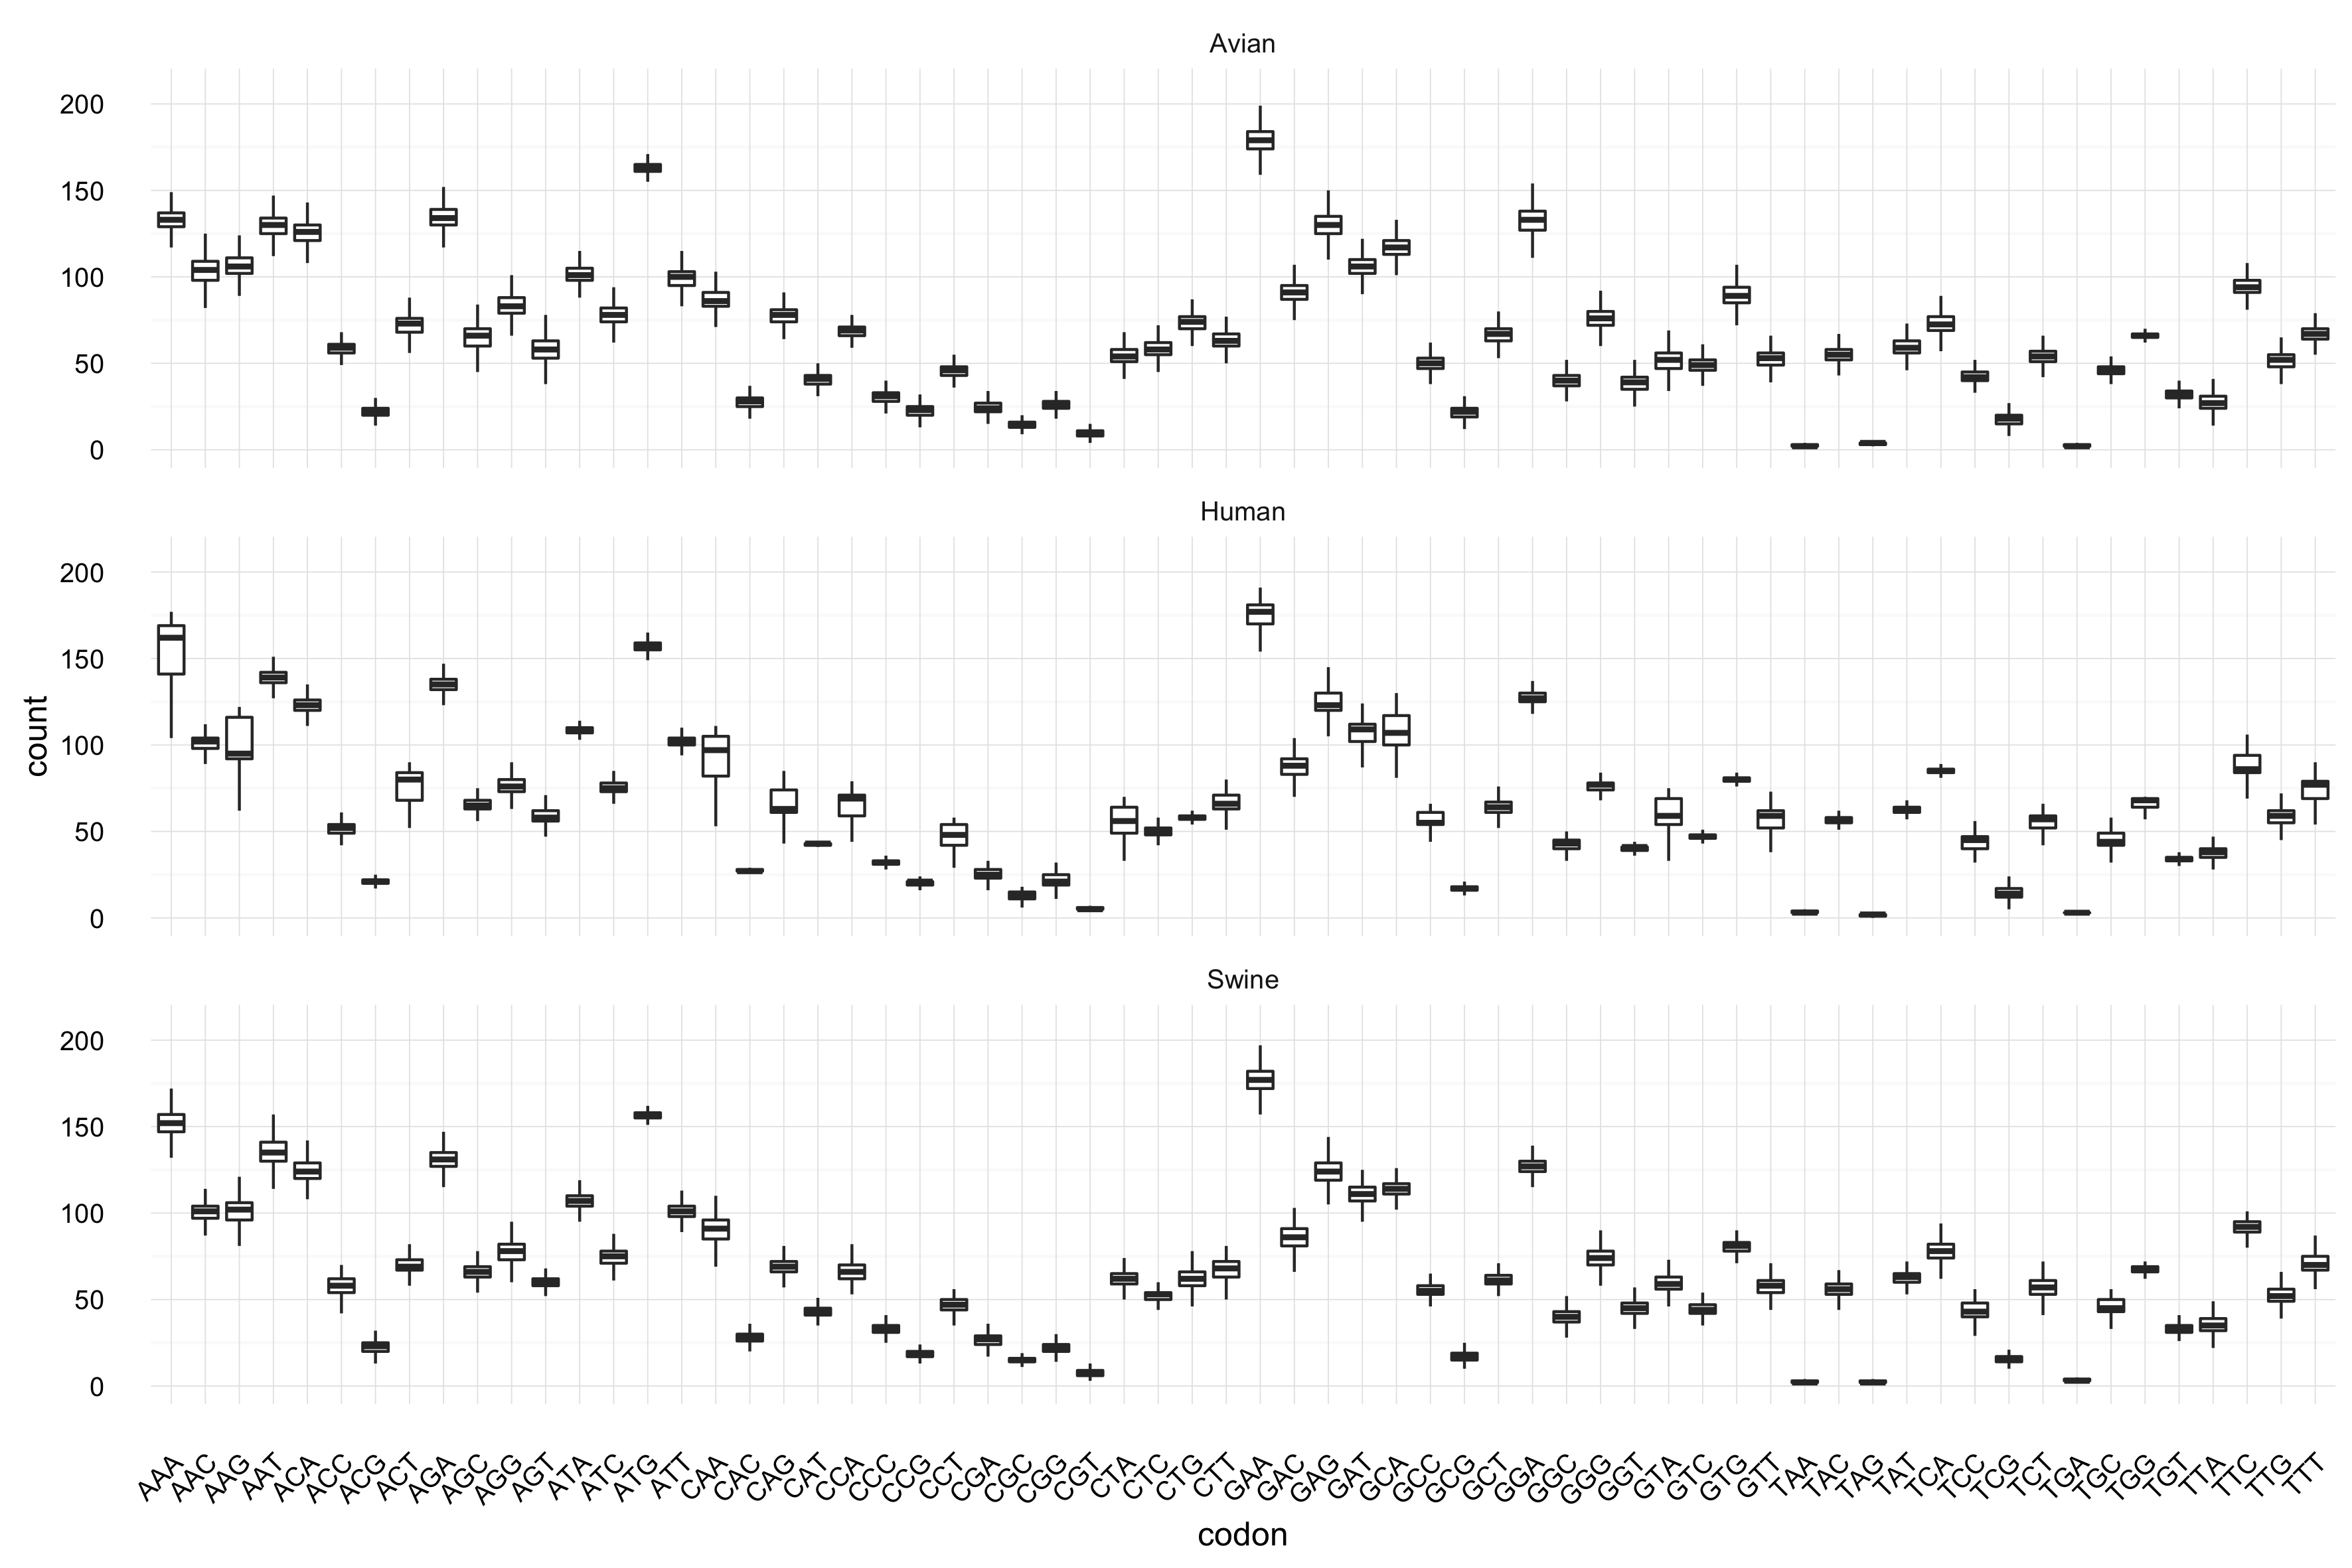
\includegraphics[scale=0.15]{boxplot_016c0.png}
    \caption[Codon usage of complete IAV genome.]{Codon usage does not show large variance accross host species (Avian, Human, Swine) as can be assessed from the boxplots accross ``columns'' in the plot facets. The x-axis displays trinucleotide combinations and the y-axis records the respective count, in aggregate referred to as codon count distribution of codon usage. Included in the analysis were 25k sequences of IAV.}
    \captionsetup{width=0.8\paperheight}
    \label{fig:distribution-codon}
\end{sidewaysfigure}


If we look at the count usage for individual segments, we can observe considerable variance between segments, but not between species (Figure \ref{fig:distribution-2nt}). We chose to plot only dinucleotides instead of codons in Figure \ref{fig:distribution-2nt} for reasons of pictorial clarity. The conclusions for di- and trinucleotides are identical. For example, comparing HA or NA to PB1, we observe a considerable drop in variance. We infer that the the nucleotide composition of segments such as PB1 is more constrained than others such as HA. One explanation is that because NA and HA are exposed to the host's immune system by being situated at the virus surface, stronger evolutionary pressures apply to mutate to escape immunity, which in turn results in greater variance of nucleotide composition. On the other end of the variance spectrum, RdRp components such as PB1 and PB2 are fundamental to virus replication and therefor more conserved.


\begin{figure}[H]
    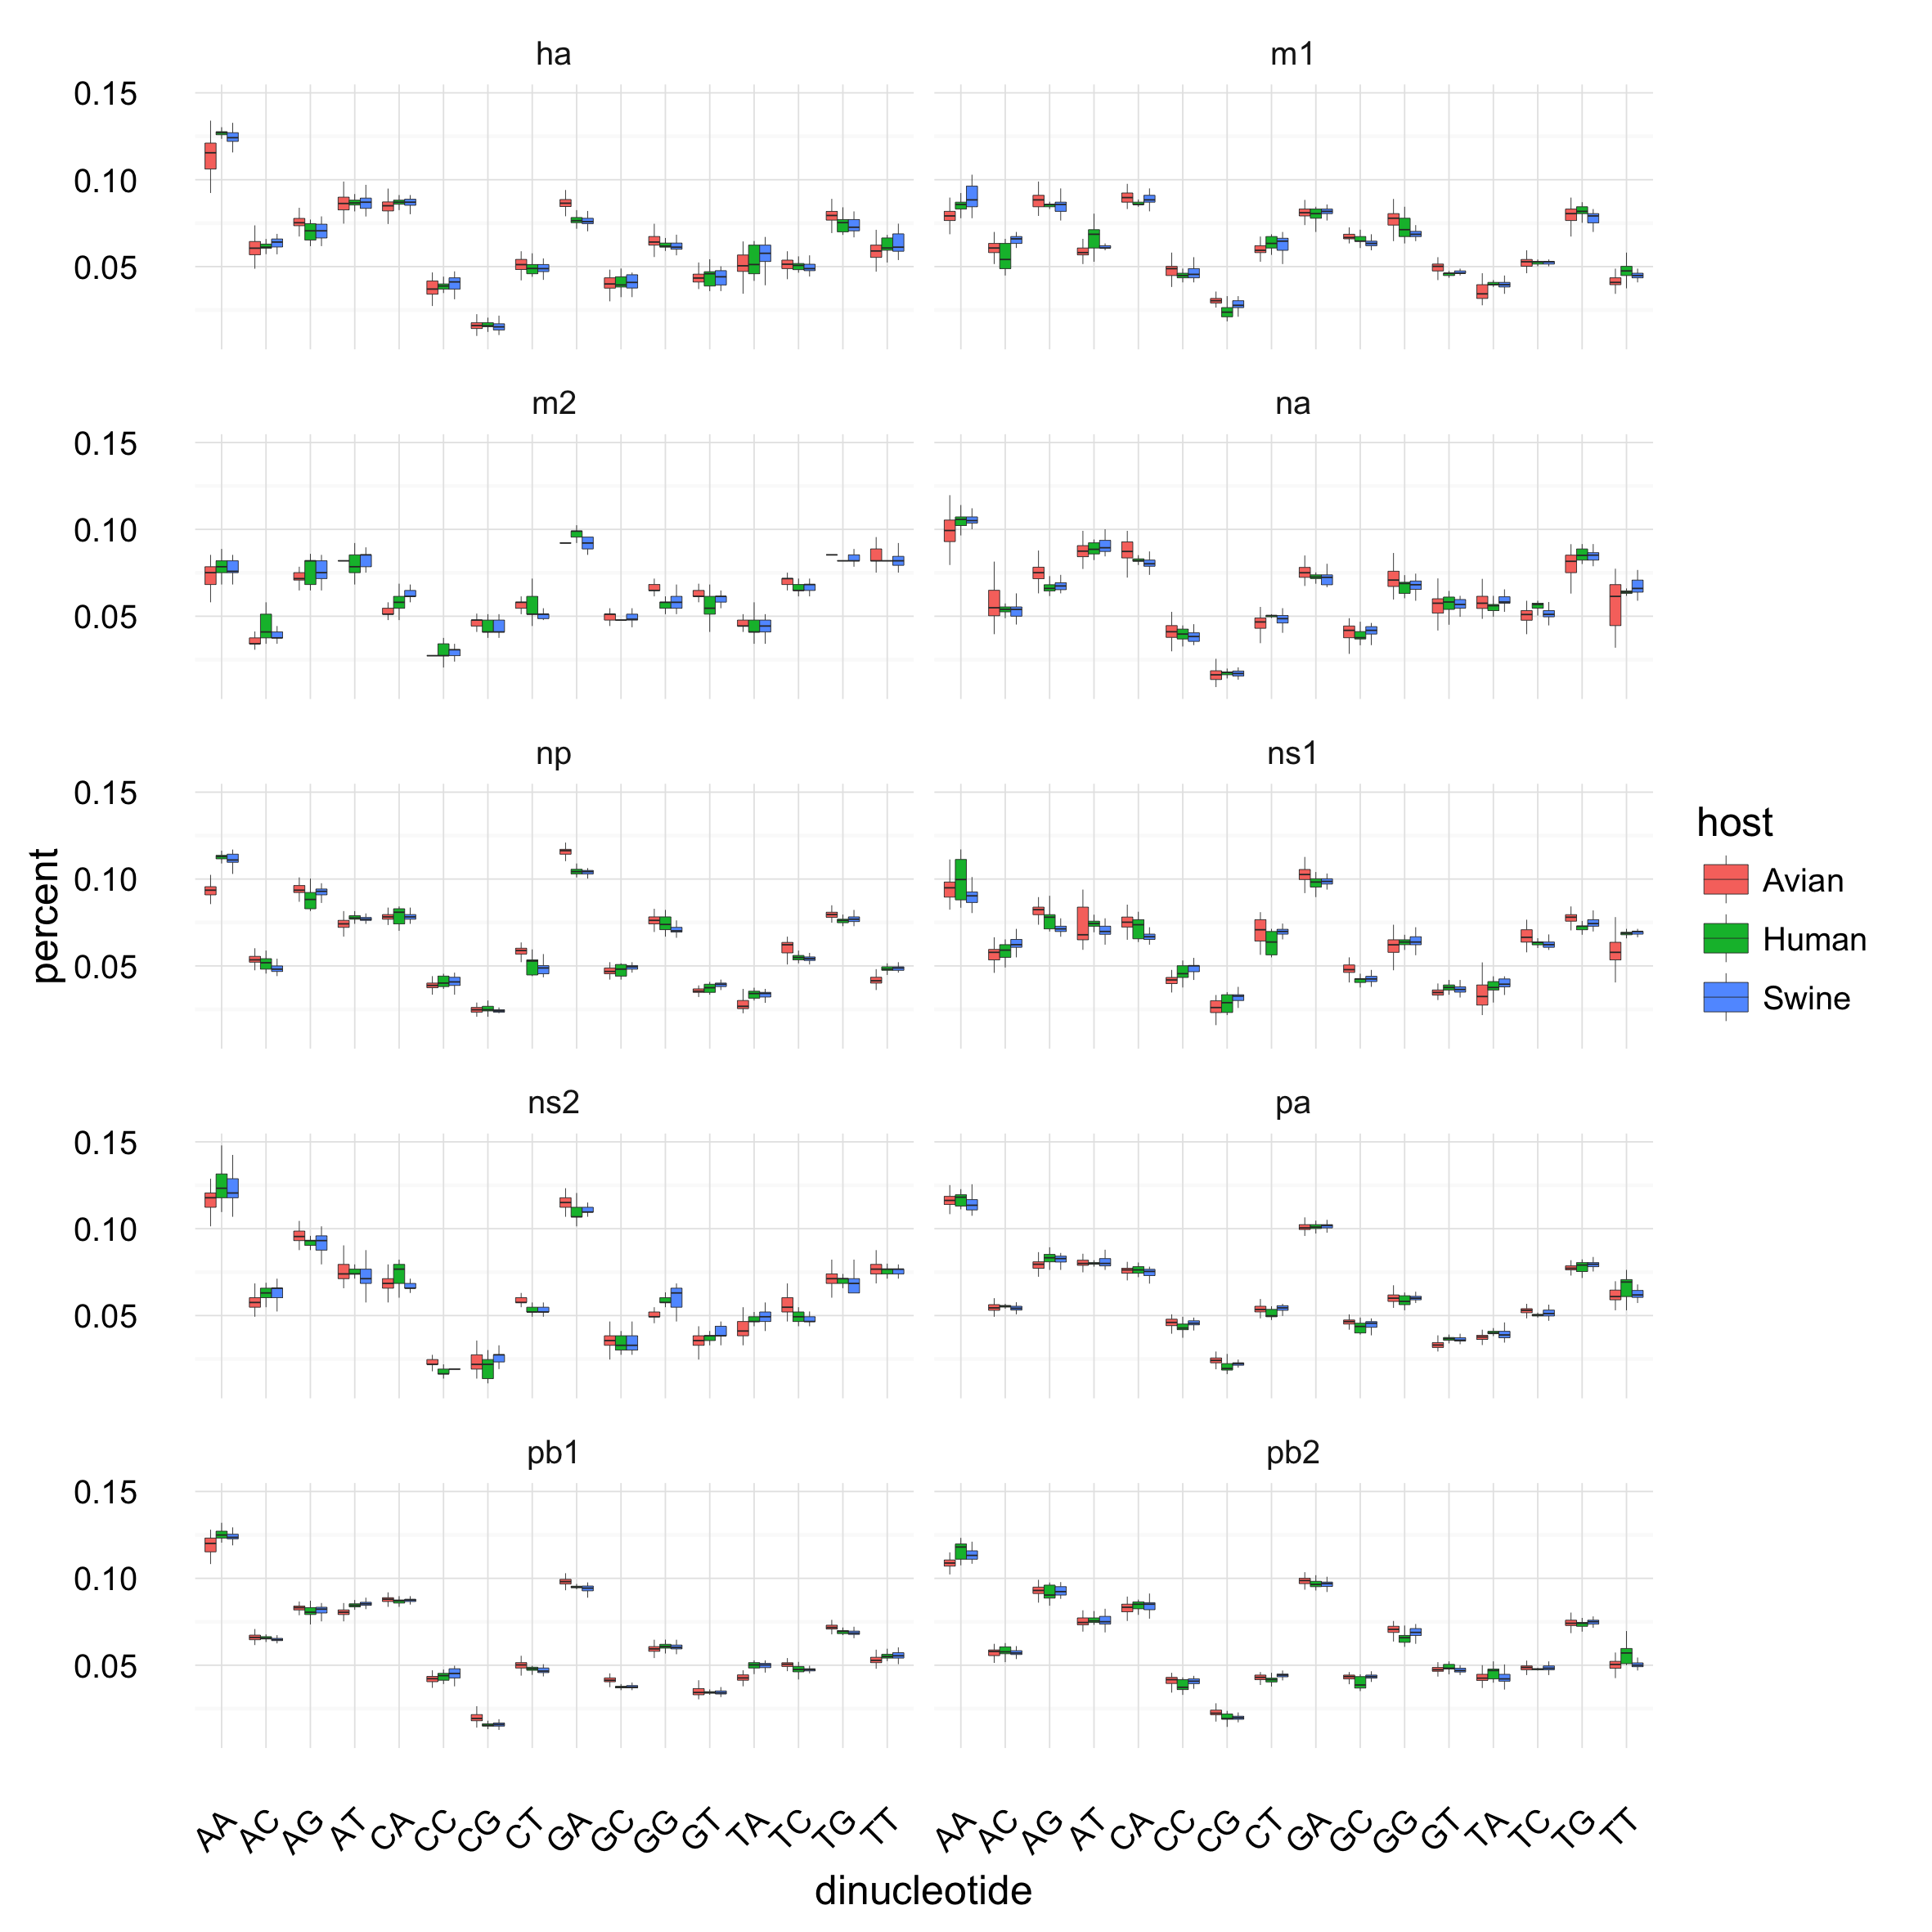
\includegraphics[scale=0.18]{kmer_2_1_segment_1d347.png}
    \caption[Dinucleotide usage of IAV genome segments.]{(Relative) dinucleotide usage differs according to IAV genome segment with plausible explanation of this observation in the different functions and constraints (see main text). Axes as in \ref{fig:distribution-codon}.}
    \label{fig:distribution-2nt}
\end{figure}


Although simply by ``eyeballing'' Figures \ref{fig:distribution-codon} and \ref{fig:distribution-2nt} one might suspect that too little variation is present to separate the sequences into distict classes. Using PCA, IAV genome samples form distinct and host-specific clusters in the first 2 principal components (Figure \ref{fig:pca1}). This means that host species can be demarcated by their (normalized) codon counts.


\begin{figure}[H]
    \begin{center}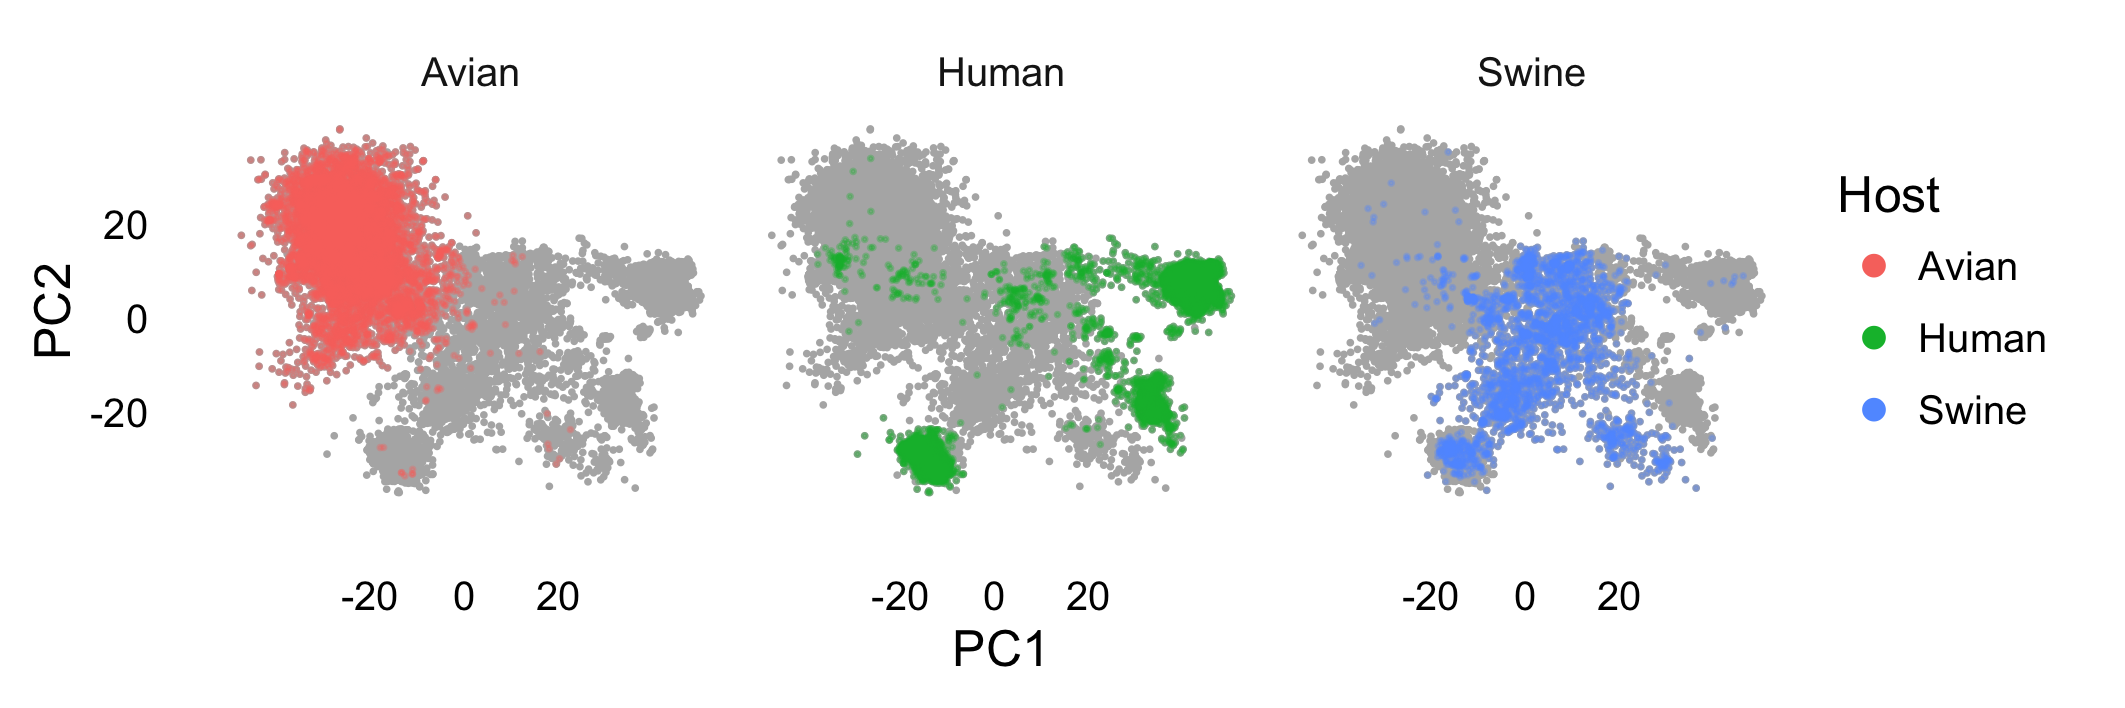
\includegraphics[scale=0.18]{pca_5b08d.png}\end{center}
    \caption[Host-specific clusters of codon usage via PCA.]{Codon usage of IAV sequences yields host-specific clusters when analysed with PCA. Principal components 1 (PC1) and 2 (PC2) are displayed (PCs are unitless). Host clusters (coloured points) have been superimposed in the respective plot facets onto the aggregate data (grey points).}
    \label{fig:pca1}
\end{figure}


More surprisingly, crudely clustering codon usage even allows the separation of various IAV subtypes. The observed clustering is hierarchical: Within ``host clusters'', IVA genome samples cluster according to their subtype (e.g. H1N1, H3N2 etc.), compare Figures \ref{fig:pca1} and \ref{fig:pca2}. We were suprised by this clear demarcation. To quantify it we used an \gls{svm}-based predictive model.


\begin{sidewaysfigure}
    \begin{center}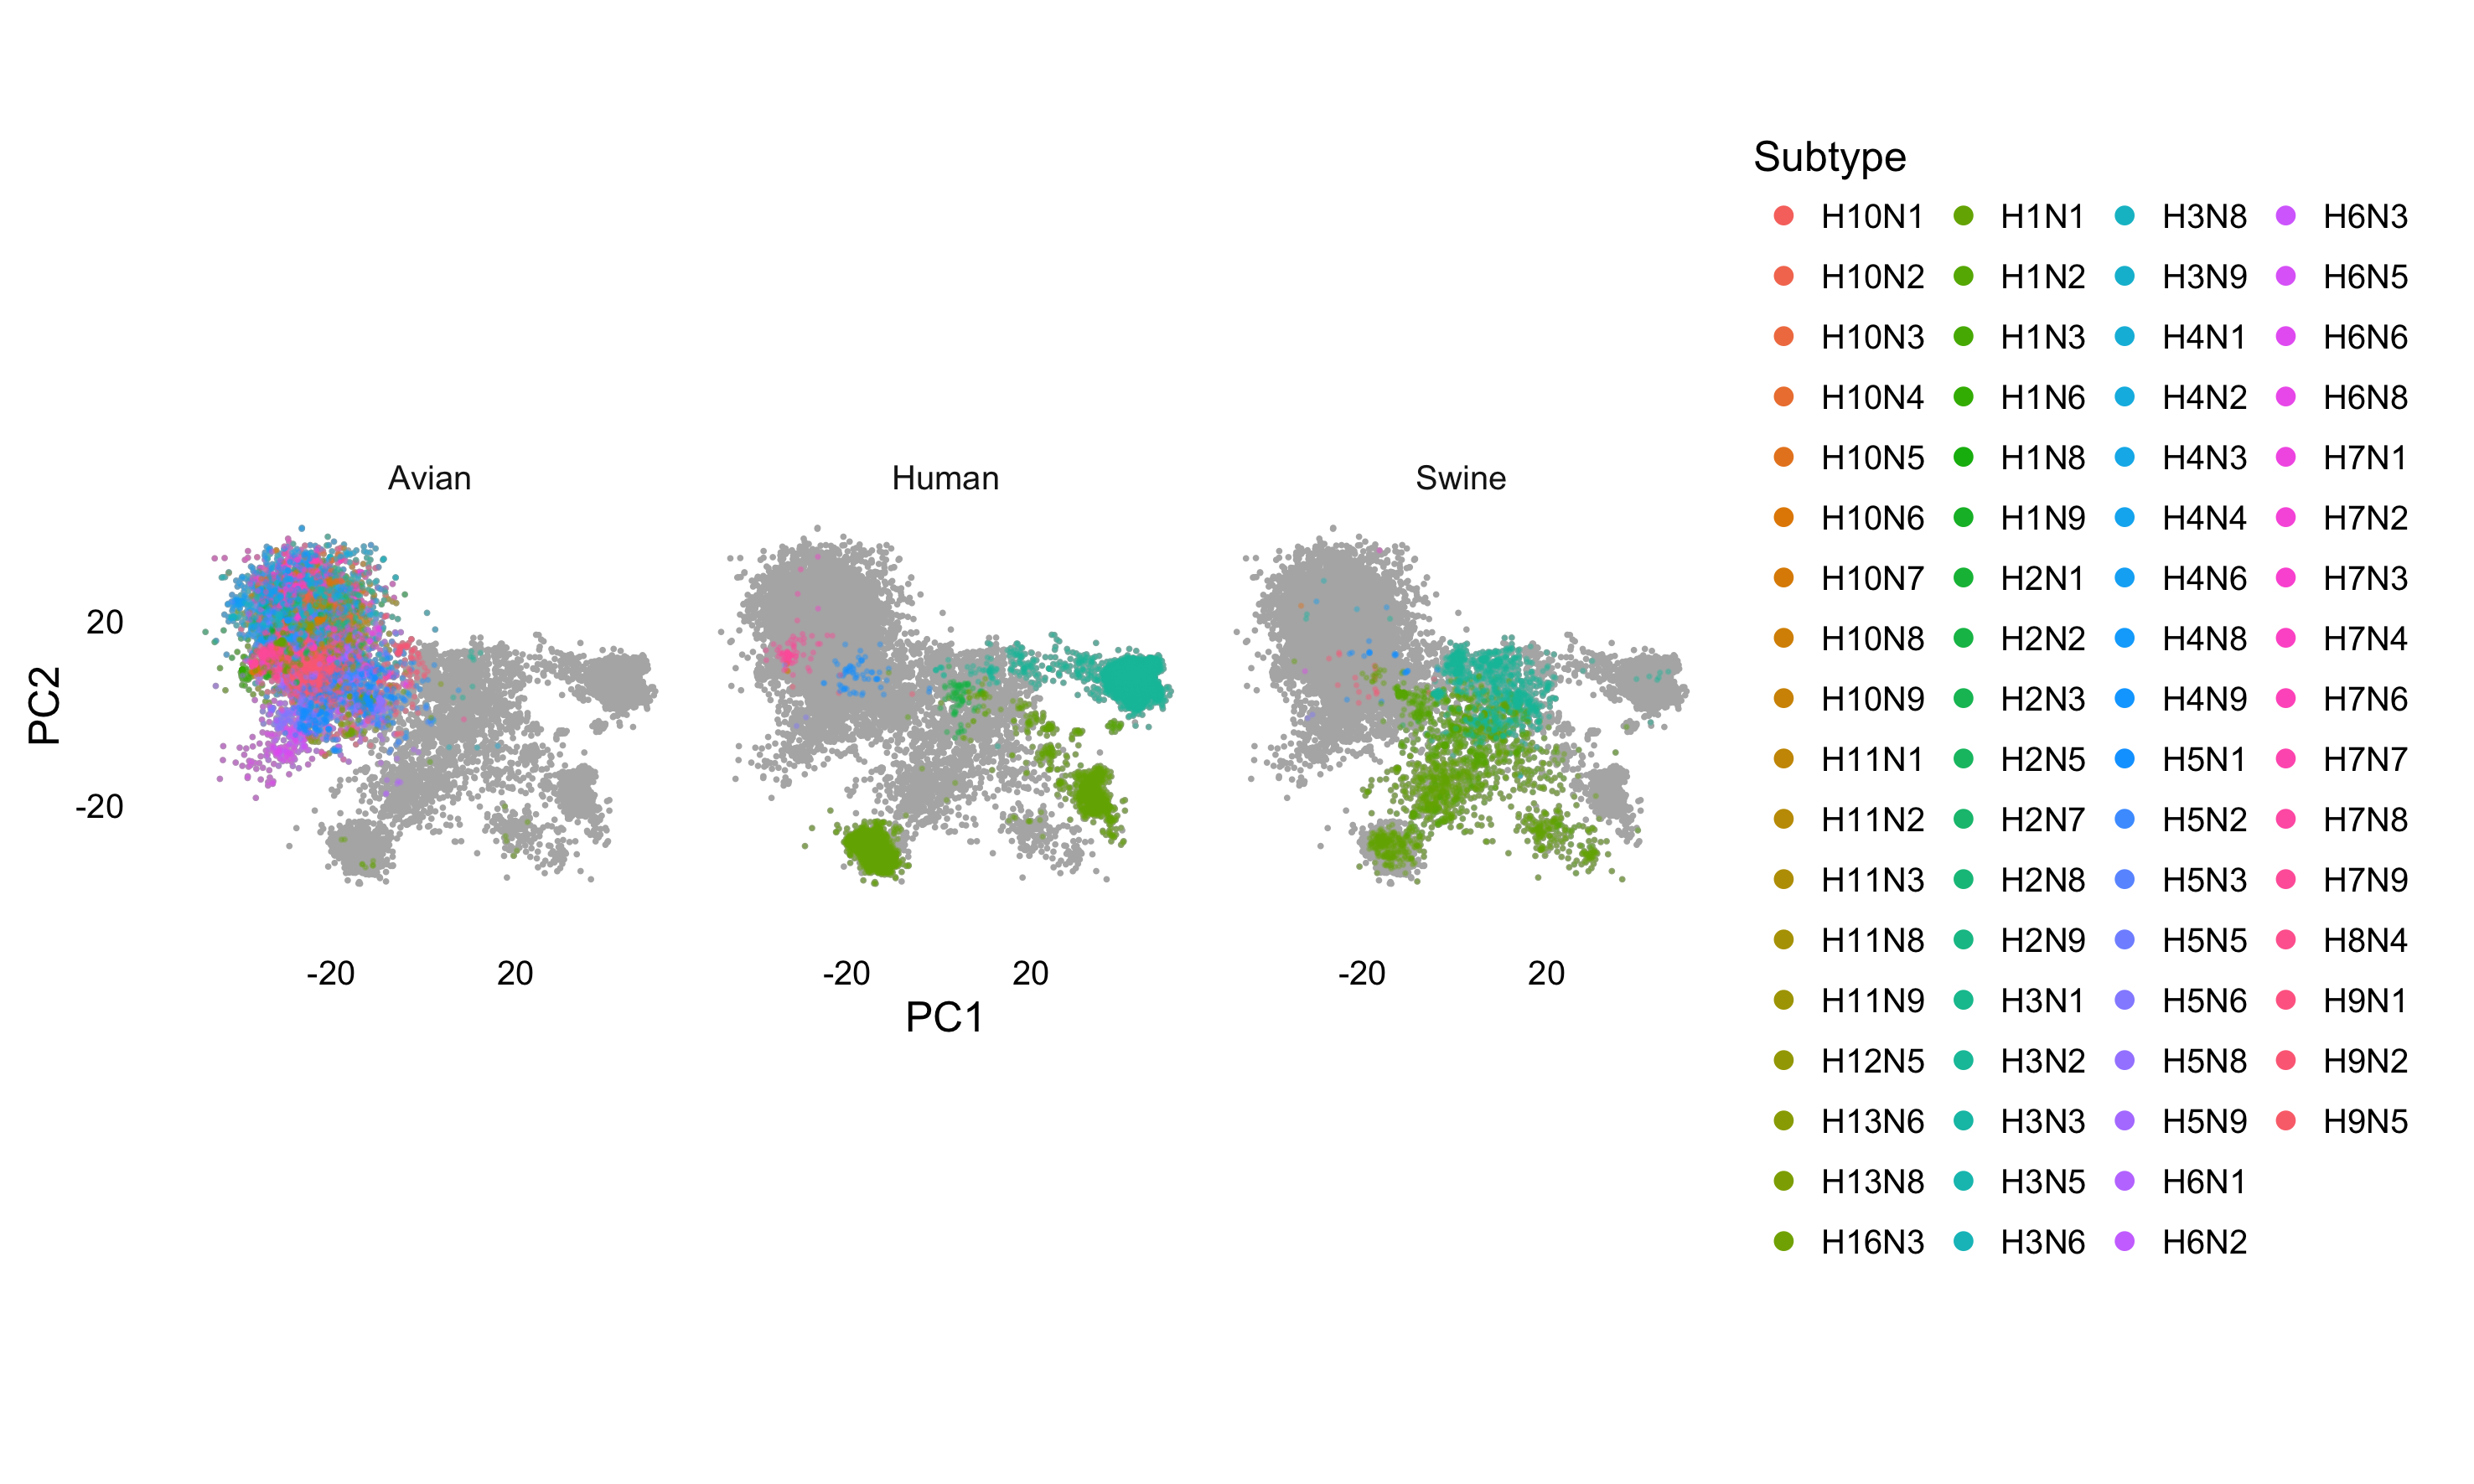
\includegraphics[scale=0.18]{pca_0dcec.png}\end{center}
    \caption[Subtype-specific clusters of codon usage via PCA.]{PCA of codon usage creates subtype specific clusters that are nested within larger host-specific clusters (compare Figure \ref{fig:pca1}). This is plausible because many subtypes prefer one host over another. Plot components are the same as in Figure \ref{fig:pca1}.}
    \label{fig:pca2}
\end{sidewaysfigure}


\subsubsection{Codon Usage Predicts Host Species with High Accuracy}

We fit an SVM based on IAV codon usage ($\hm{X}$) for 15k samples. This constitutes the balanced training set with 5k samples for each host (i.e. a stratified sample). Host labels (Avian, Human, Swine) were used as prediction target $\hm{y}$. This setup produced very good predictive results (Table \ref{tab:confusion-main} and \ref{tab:modeleval}): We could predict the correct host label for input sequences with an overall accuracy of 95\%. Our method's sensitivity (recall) was 99\% with an overall positive predictive value (precision) of about 92\%.


\begin{table}[htbp]
    \centering
    \begin{tabular}{c | c | c | c | c}
        $\hm{y}$ \textbackslash~$\hm{\hat{y}}$ & Avian & Human & Swine & All \\
        \hline
        Avian   & 3207  & 49    & 13    & 3269 \\
        Human   & 6     & 4470  & 82    & 4558 \\
        Swine   & 9     & 10    & 849   & 868  \\
        All     & 3222  & 4529  & 944   & 8695 \\
    \end{tabular}
    \caption[SVM classifier: Confusion matrix.]{Confusion matrix of the SVM classifier, where true $\hm{y}$ and predicted $\hm{\hat{y}}$ hosts are tabulated. For example, of a total of 3222 Avian samples, 3207 were correctly assigned to class Avian, while 6 and 9 were wrongly assigned to Human and Swine, respectively.}
    \label{tab:confusion-main}
\end{table}


% This table somehow causes compilation problems. Fix later if necessary.
\begin{table}[htbp]
    \centering
    \begin{tabular}{c | c | c | c | c}
        metric \textbackslash~host & Avian & Human & Swine &  All \\
        \hline
        accuracy & \phantom{} & \phantom{} & \phantom{} & 0.95 \\
        recall & 0.99 & 0.95 & 0.94 & \phantom{} \\
        precision & 0.88 & 1 & 0.89 & \phantom{} \\
        F1-score & 0.94 & 0.97 & 0.93 & \phantom{} \\
    \end{tabular}
    \caption[Model evaluation according to 4 standard metrics.]{Model evaluation according to 4 standard metrics. Overall, the SVM classifier is both very sensitive and specific.}
    \label{tab:modeleval}
\end{table}


We wanted to investigate what information the SVM actually used to make predictions, i.e. which aspects of the codon usage allow the separation of host classes. We refit the SVM to dinucleotide counts as well as to trinucleotide counts with an offset of 1 nt, so as to count trinucleotides but not codons. We restricted the analysis to the coding sequence of the HA protein because this sequence has the largest nucleotide entropy accross samples in the MSA (Figure \ref{fig:distribution-2nt}). We contrained the SVM to train on only 1k samples so that the resulting model generalizes better (i.e. is less prone to overfitting). As a side effect, the required computational load dropped substantially by about an order of magnitude.

As is to be expected, the performance of this model is not as good because we only used 1k samples during training (Table \ref{tab:confusion-3nt}). Interestingly, dinucleotide usage (Table \ref{tab:confusion-2nt}) is enough to assign the correct host in many cases, which is surprising, given that the distribution does not vary much between species (Figure \ref{fig:distribution-2nt}). Generally, separation between Avian an Mammalian classes does not seem to be a problem for the SVM, but distinguishing Human and Swine host species is.


\begin{table}[htbp]
    \centering
    \begin{tabular}{c | c | c | c | c}
        $\hm{y}$ \textbackslash~$\hm{\hat{y}}$ & Avian & Human & Swine & All \\
        \hline
        Avian   & 5524  & 227    & 576    & 6327 \\
        Human   & 168   & 11314    & 1251   & 12733 \\
        Swine   & 25    & 800     & 995   & 1820  \\
        All     & 5717  & 12341   & 2822   & 20880 \\
    \end{tabular}
    \caption{Model evaluation for codon usage.}
    \label{tab:confusion-3nt}
\end{table}


\begin{table}[htbp]
    \centering
    \begin{tabular}{c | c | c | c | c}
        $\hm{y}$ \textbackslash~$\hm{\hat{y}}$ & Avian & Human & Swine & All \\
        \hline
        Avian   & 4294  & 1048    & 985    & 6327 \\
        Human   & 173   & 8376    & 4184   & 12733 \\
        Swine   & 17    & 630     & 1173   & 1820  \\
        All     & 4484  & 10054   & 6342   & 20880 \\
    \end{tabular}
    \caption{Model evaluation for dinucleotide usage.}
    \label{tab:confusion-2nt}
\end{table}


\begin{table}[htbp]
    \centering
    \begin{tabular}{c | c | c | c | c}
        $\hm{y}$ \textbackslash~$\hm{\hat{y}}$ & Avian & Human & Swine & All \\
        \hline
        Avian   & 5519  & 408    & 400    & 6327 \\
        Human   & 201   & 6152    & 6380   & 12733 \\
        Swine   & 34    & 557     & 1229   & 1820  \\
        All     & 5754  & 7117   & 8009   & 20880 \\
    \end{tabular}
    \caption{Model evaluation for frameshift codon usage.}
    \label{tab:confusion-frameshift}
\end{table}


When we introduce a frameshift in the trinucleotide count (Table \ref{tab:confusion-frameshift}), we are no longer able to separate the human and swine classes. This is interesting because it means that codon bias is at least partly informative in the separation of host species, and it suggest a hierarchical model: The destinction between mammal and bird thus stems largely from k-mer frequency, but between closely related species such as human and swine, the SVM likely draws its information from codon bias.


\newpage\subsection{Analysis of Experimental Codon Bias}

Next we turned to an ML technique called \gls{gbt}. We chose this technique over SVM because the latter offer very little insight into why a particular classification was learned the way it was, i.e. SVMs are a rather black box. GBMs on the other hand are very transparent, because they are built from decision trees. These recursively split the data set: At each node of the split one can follow which decision was taken.


\subsubsection{Learning Host-Specific Loci Consistently using GBTs}

First, we wanted to verify that the GBT algorithm yields consistent results. From the \gls{iav} MSA we selected 100 positions at random to test this. With 2k one-hot encoded samples for each of the 3 host labels (Avian, Human, Swine) the resulting feature matrix had dimensionality $6(10^3) \times 400$. We ran predictions on a balanced test set of 1k samples for each host label. Then we repeated this process 20 times and logged the position-wise \gls{fi} score.

The resulting predictions are displayed in Figure \ref{fig:consistency} and are very consistent accross the 20 trials, i.e. the same positions are assigned approximately the same \gls{fi}. Random aspects of the GBT algorithm do not seem to cause different results when given the same input data.


\begin{figure}[H]
    \begin{center}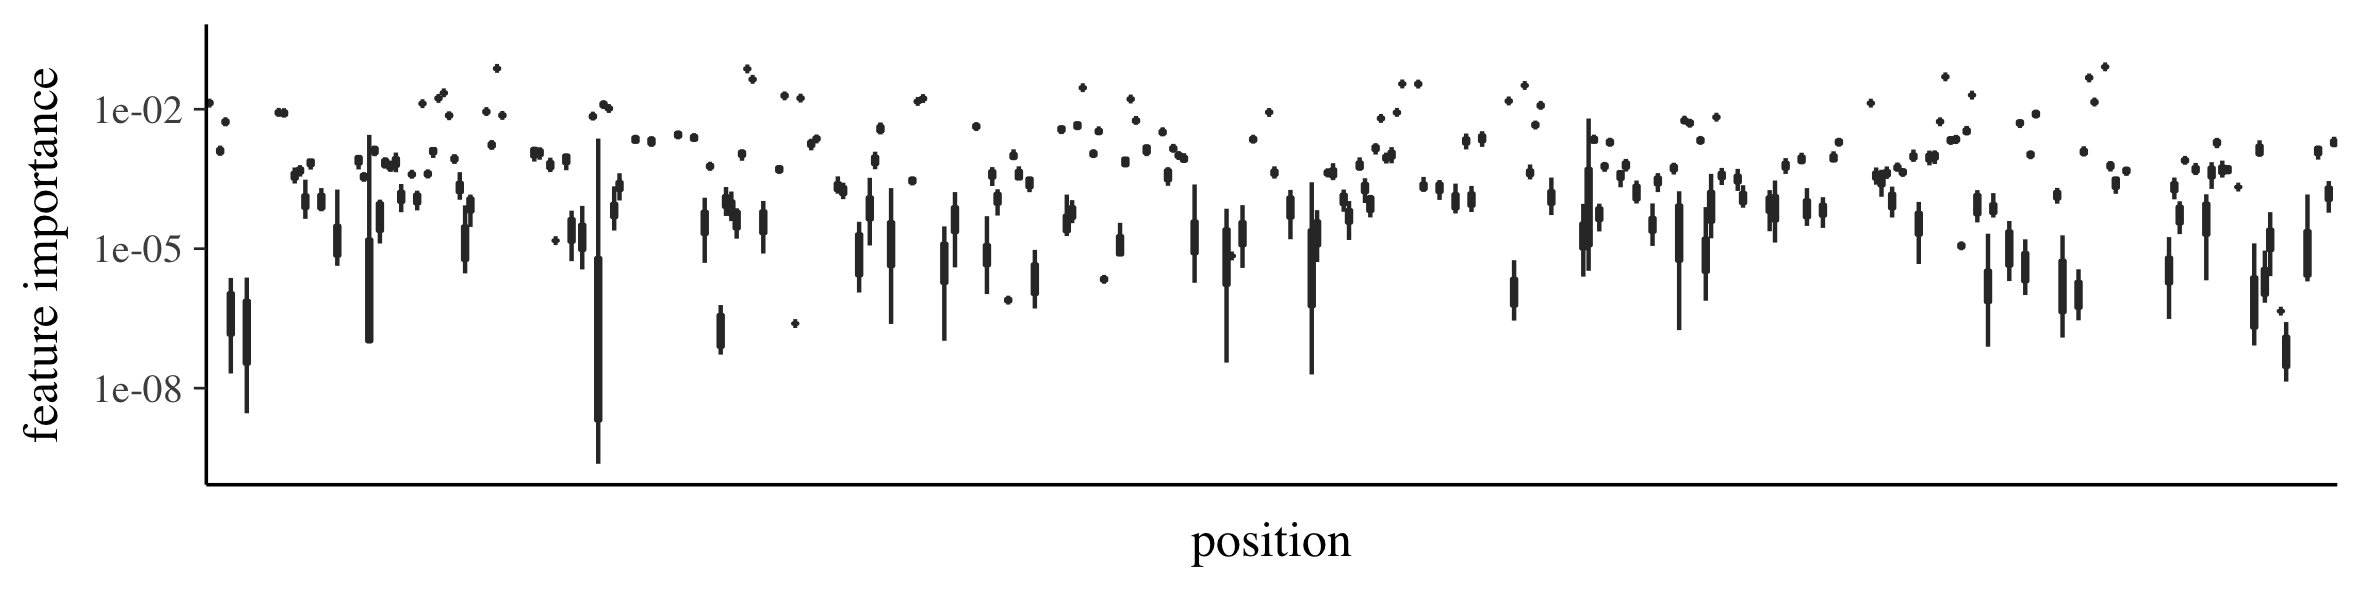
\includegraphics[scale=0.18]{PA_random100_repeat20_log.png}\end{center}
    \caption[GBTs assign consistent feature importances to tested loci.]{GBTs assign consistent feature importances to tested loci. The boxplot shows log feature importance on the y axis with loci being indexed on the x-axis. Note that because we one-hot encoded the nucleotide sequences, 4 positions in the index correspond to one position in the sequence. We observe very consistent learning behaviour from the GBTs with many irrelevant features being shrunken towards 0.}
    \label{fig:consistency}
\end{figure}


We then wondered whether the signal picked up by the GBTs is the entropy in each column of the MSA, i.e. the position-wise information. Figure \ref{fig:entropy-scatter} shows a scatter plot of the positional entropy along the PA gene of IAV. Note that while there seem to be 2 ``bands'' $y=\{0, 1\}$, the entropy distribution along the gene seems homogenous, i.e. we do not observe any entropy (i.e. mutational) hot spots.


\begin{figure}[H]
    \begin{center}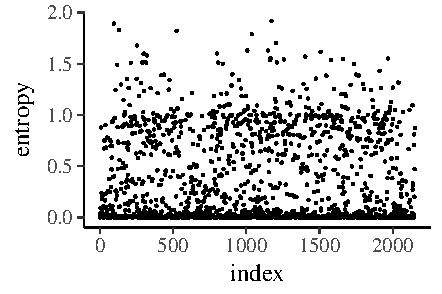
\includegraphics[scale=1]{entropy_PA_train_test.pdf}\end{center}
    \caption[Entropy of loci along PA segment.]{Entropy of loci (index) along PA segment. The entropy distribution along the PA gene seems homogenous without any obvious mutational hot spots.}
    \label{fig:entropy-scatter}
\end{figure}


The observed bands correspond to a bimodal entropy distribution with 2 modes around 0 and 1 (see Figure \ref{fig:entropy-freqpoly}). Note that when H = 0, all nucleotides at a particular locus are of the same type, i.e. the site is perfectly conserved.


\begin{figure}[H]
    \begin{center}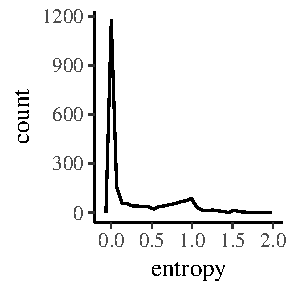
\includegraphics[scale=1]{entropy_PA_freqpoly.pdf}\end{center}
    \caption[Bimodal entropy distribution.]{We can observe a bimodal entropy distribution H. When H = 0 for a given locus, all sequences present the same nucleotide at this index. When H = 1, we observe only 2 nucleotides at this locus at a ratio of 1:1.}
    \label{fig:entropy-freqpoly}
\end{figure}


We then correlated entropy to feature importance for all loci with FI $> 5(10^{-4})$. We observed a roughly log-linear relationship (Figure \ref{fig:correlation}), although we did not quantify it. This relationship is plausible: a locus that is more informative from an information theoretic standpoint seems to be more important in the learning process.


\begin{figure}[H]
    \begin{center}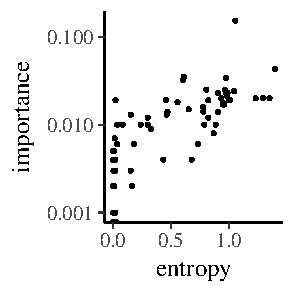
\includegraphics[scale=1]{entropy_PA_feat_importance.pdf}\end{center}
    \caption[Log linear relationship between entropy and feature importance.]{There is an approximate log-linear relationship between entropy and feature importance. Note however that we observe some loci which do not hold much information but nevertheless are important for classification. Those are likely host-specific minor variants, although we did not investigate this matter further.}
    \label{fig:correlation}
\end{figure}


Because entropy seemed very important for the predictive performance of the GBTs, we wanted to verify that the way we split our data set into a test and training sample (stratified) does not introduce an entropy bias. Figure \ref{fig:delta} confirms that this is not the case.


\begin{figure}[H]
    \begin{center}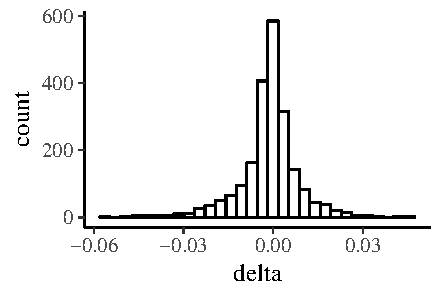
\includegraphics[scale=1]{entropy_PA_delta.pdf}\end{center}
    \caption[No entropy bias in test-train split.]{No entropy bias is present after the data set has been split into a test and training set. We calculated the position-wise difference between the test and training set and plotted the resulting histogram. Note how the entropy difference does not deviate substantially from 0.}
    \label{fig:delta}
\end{figure}


After these experiments we were confident that GBTs offered consistent performance on our learning problem. We next applied them to sequences that were subject to codon deoptimization.


\subsubsection{Inconsistent Feature Importance for Deoptimized Loci}

We analysed a total of 8 samples (including wild type) of Influenza virus A genomes that had been modified through strategies of codon deoptimization (Table \ref{tab:deopt-experiments}). The \gls{na} genes of IAV strain A/WSN/1933 (H1N1) were recoded (see methods section for protocol details). More specifically, the \gls{orf} was recoded between nucleotides 184-1200, such that 120 nt on both ends were left intact. Only non-terminal parts of the gene were targeted, because the 5'- and 3'- terminus sequences are important during IAV packaging: When the termini are deoptimized, no viable virions assembly fails (D. Kunec, personal communication).

To summarize Table \ref{tab:deopt-experiments}, the WT, DL, DM, HS, OG, and PD variants have the same codon bias (i.e. they contain the same codons) and are mainly distinguished by their \gls{cpb}. The H and HD have a different codon bias because they were designed with the aim of maximizing the GC content, where maximizing means iterative sequence changes up to a threshold above which no viable virions could be obtained.


\begin{table}[htbp]
    \centering
    \begin{tabularx}{\textwidth}{l | r | c | l | X}
        label & CPB & plaque size & name & description \\
        \hline
        WT & 0.004 & 1.00 & wild type & \\
        DL & -0.231 & 0.31 & deoptimized-less & codon pair deoptimized, less \\
        DM & -0.449 & 0.11 & deoptimized-more & codon pair deoptimized, more \\
        HS & -0.049 & 0.94 & high-score & same number of NNC-GNN codon pairs as in DM, and codon pair \\
        OG & -0.209 & 0.99 & optimized-good & same NNC-GNN codon pairs as in DM, and codon pair \\
        PD & -0.222 & 0.35 & pure deoptimization & same NNC-GNN codon pairs as in WT, and codon pair \\
        H & -0.207 & 0.52 & high & CpG maximized \\
        HD & -0.339 & 0.39 & high deoptimzed & CpG maximized and codon pair deoptimized \\
    \end{tabularx}
    \caption[Summary of deoptimized sequences.]{Summary of the deoptimization experiments. 7 deoptimized variants were constructed from 1 wild type IAV strain A/WSN/1933 (H1N1). CPB: codon pair bias, plaque size: a measure of virus viability/ attentuation (smaller means more attentuated).}
    \label{tab:deopt-experiments}
\end{table}


We then marked the deoptimized positions in a scatter plot of the previously learned feature importances (Figure \ref{fig:feature-importance}). We hypothesized that virus variants where \gls{na} loci of high \gls{fi} had been deoptimized would result in a more attenuated phenotype. However, no consistent signal could be observed: While some loci with high FI have been targeted by the deoptimization, we could observe no clear link between the FI of targeted loci and the resulting viability phenotype of the 7 IAV variants.

Note that the deoptimized sequences had already been designed with more or less heuristic principles before we started our investigation, so that our analysis was retrospective and did not inform the deoptimization targets priori.


\begin{SCfigure}
  \centering
  \caption[Deoptimized loci mapped to learned feature importances.]{Deoptimized loci mapped to learned feature importances for the ``DL'' variant (other variants not shown). The position-wise FI (light red) was learned from the above described host species prediction task using GBTs. We then superimposed the loci that had been subject to codon deoptimization (in dark red). While some loci with high FI have been targeted, we could observe no clear link between the FI of targeted loci and the resulting viability phenotype of the IAV variants (see plaque score in Figure \ref{tab:deopt-experiments}). FI is scaled by square root ($\sqrt{F}$) for easier visual inspection. Modified label 0: no, 1: yes, i: index. Note that the 4 facets \{A, C, T, G\} result from the one-hot encoding, where each sequence locus is transformed into 4 features. Each of those features could be informally translated as asking: ``Is a given nucleotide present at this locus?''.}
  \label{fig:feature-importance}
  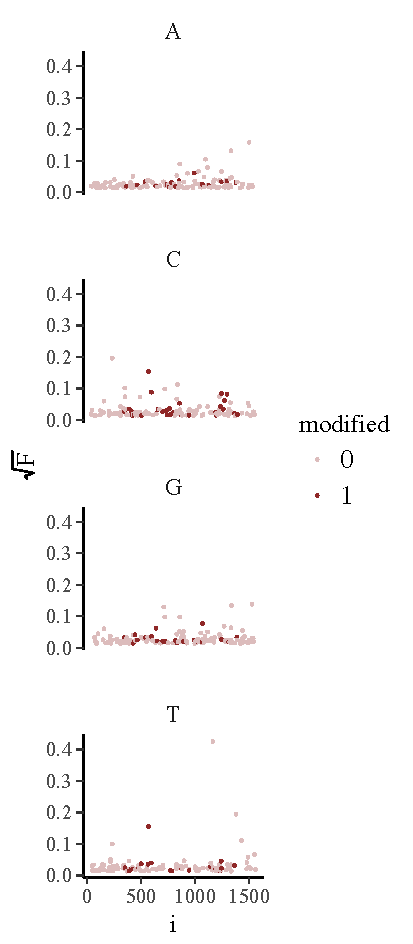
\includegraphics[scale=1]{NA_fi_deopt.pdf}
\end{SCfigure}


\begin{figure} % [H]
    \begin{center}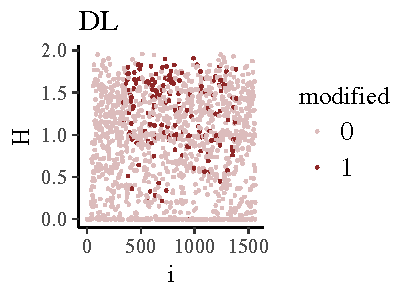
\includegraphics[scale=1]{NA_h_deopt.pdf}\end{center}
    \caption[Deoptimized loci marked in a scatter plot of entropy and index position.]{Deoptimized loci marked in a scatter plot of entropy and index position for DL variant of IAV. We can appreciate how only ``internal'' loci have been targeted by the deoptimization (color code as in Figure \ref{fig:feature-importance}). However, the deoptimization does not target high entropy loci specifically.}
    \label{fig:entropy}
\end{figure}


Similarly we did not observe a clear pattern concerning deoptimized loci with respect to entropy (Figure \ref{fig:entropy}).


\newpage


\subsection{zoo - A New Data Structure for the Exchange of (Viral) Data}

\begin{quotation}
\emph{Simplicity is a prerequisite for reliability.\\
-- E. Dijkstra}
\end{quotation}

\vspace{0.5cm}

\begin{quotation}
\emph{Equating simplicity with ease and familiarity is wrong.\\
-- R. Hickey}
\end{quotation}

\vspace{0.5cm}

The zoo software package is available at \hyperlink{https://github.com/viehwegerlib/zoo}{github.com/viehwegerlib/zoo} with detailed information on installation and usage as well as related background information in the form of a wiki. zoo can be cited under \colorbox{red-very-light}{\lstinline{doi.org/10.5281/zenodo.801560}}.

zoo is a tool to compose and manipulate units of sequence data in the form of so-called data cells, as well as a protocol to exchange them. Data cells are intended to be shared through a decentralized \gls{p2p} network, implementing an offline first design. A data cell's sequence content can be seached efficiently via Minhash signatures.


\subsubsection{Desiderata}

We pose three desiderata of a data structure in microbial bioinformatics:

First, it needs to have a rich data structure, e.g. allowing entries to be nested and/ or linked. This is necessary to represent biological data, which in spite of curative efforts remain mostly messy. The trend towards more entropy is likely to continue, while curative resources remain flat.

Second, the data structure needs a well designed \gls{api}, which allows complex queries. Ideally, it would also offer convenience functions to combine data in informative ways. For example, we would like to query sequence data by taxonomy as well as phylogeny. The API should link to downstream analyses with third party tools, e.g. for multiple sequence alignments and machine learning.

Third, we likely need to share data with collaborators and other stakeholders. Thus, the data structure needs to be implemented in a highly portable way, including easy and quick setup/ deletion as well as version control. The data structure is created for usage in the context of a project, and can be discarded after usage, while logging all the steps needed to recreate it if need be.


\subsubsection{An Atomic Unit of Data}

We termed the atomic unit of data in zoo a ``data cell''. We will leave definitions and implementation details for later and focus for now on a high-level description. A data cell is used to encapsulate the data in a sort of container and expose it to the outside world through a set of interfaces, which are provided by zoo.

zoo itself has two components: a (largely Python) library and a database engine. The engine stores and internally manages the data cell, and the library allows the user to work on the data through the interface.

Data cells can be composed like lego blocks. For example, a given curated data cell on flaviviruses can be updated with new experimental results. One could imagine such data cell composites to be directly attached to a publication, especially when a lot of new sequence data has been generated.


\subsubsection{The Data Cycle}

To use an abstraction, a data cell is a relay: Data from experiments or databases is distributed between collaborators and to and from downstream analyses (Figures \ref{fig:nz1} and \ref{fig:nz2}).


\begin{figure}[H]
    \begin{center}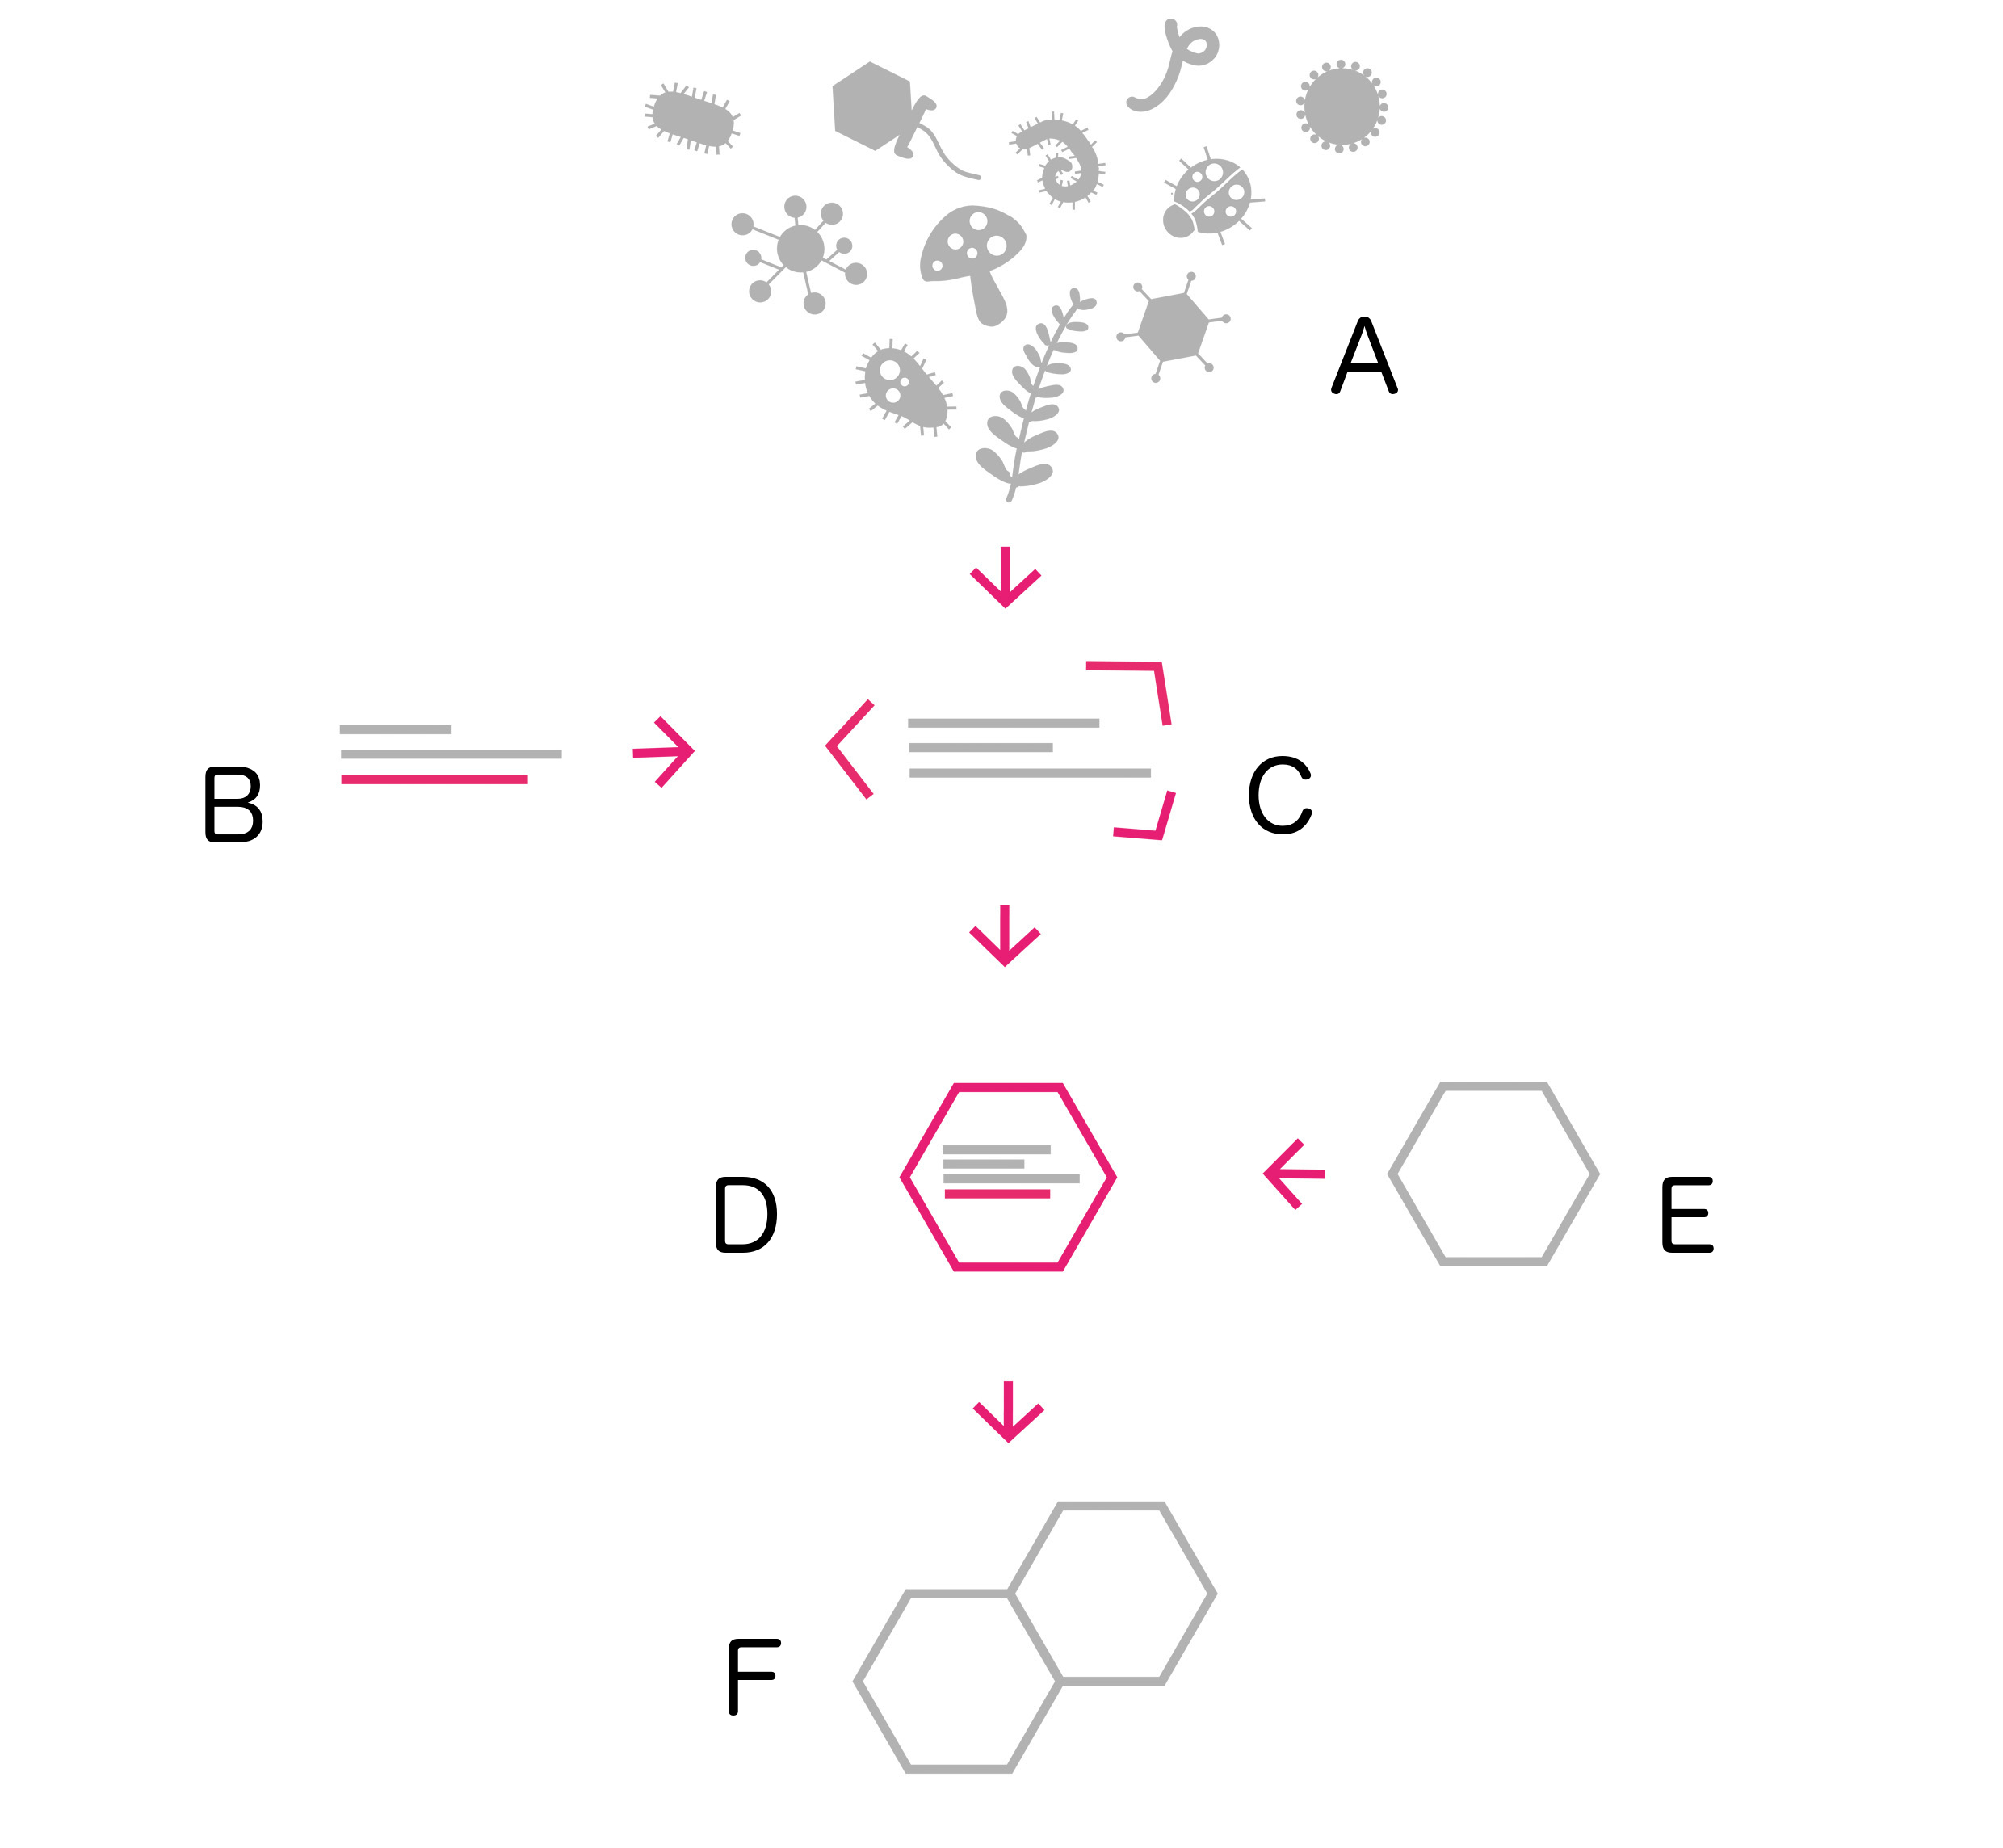
\includegraphics[scale=0.35]{nanozoo_broschuere_abwandlung_a4_part1_wletters.jpeg}\end{center}
    \caption[Infographic: Loading data into a data cell.]{Loading data into a data cell. Sample sequences - DNA, RNA or protein (A) - are combined with comparative sequences from databases (B) and ``containerized'' (C). This import process employs schemas to structure the data in predefined ways and to allow input validation. The whole construct is made accessible to the outside world through an interface. This process generates a data cell (D). Data cells can be composed with other data cells into composites (D + E = F), which implement the same set of interfaces and aim to be data backends that plug into downstream analyses (see Figure \ref{fig:nz2}).}
    \label{fig:nz1}
\end{figure}


By using the proposed protocol, data undergoes a sort of cycle (Figure \ref{fig:circle}).


\begin{figure}[H]
    \begin{center}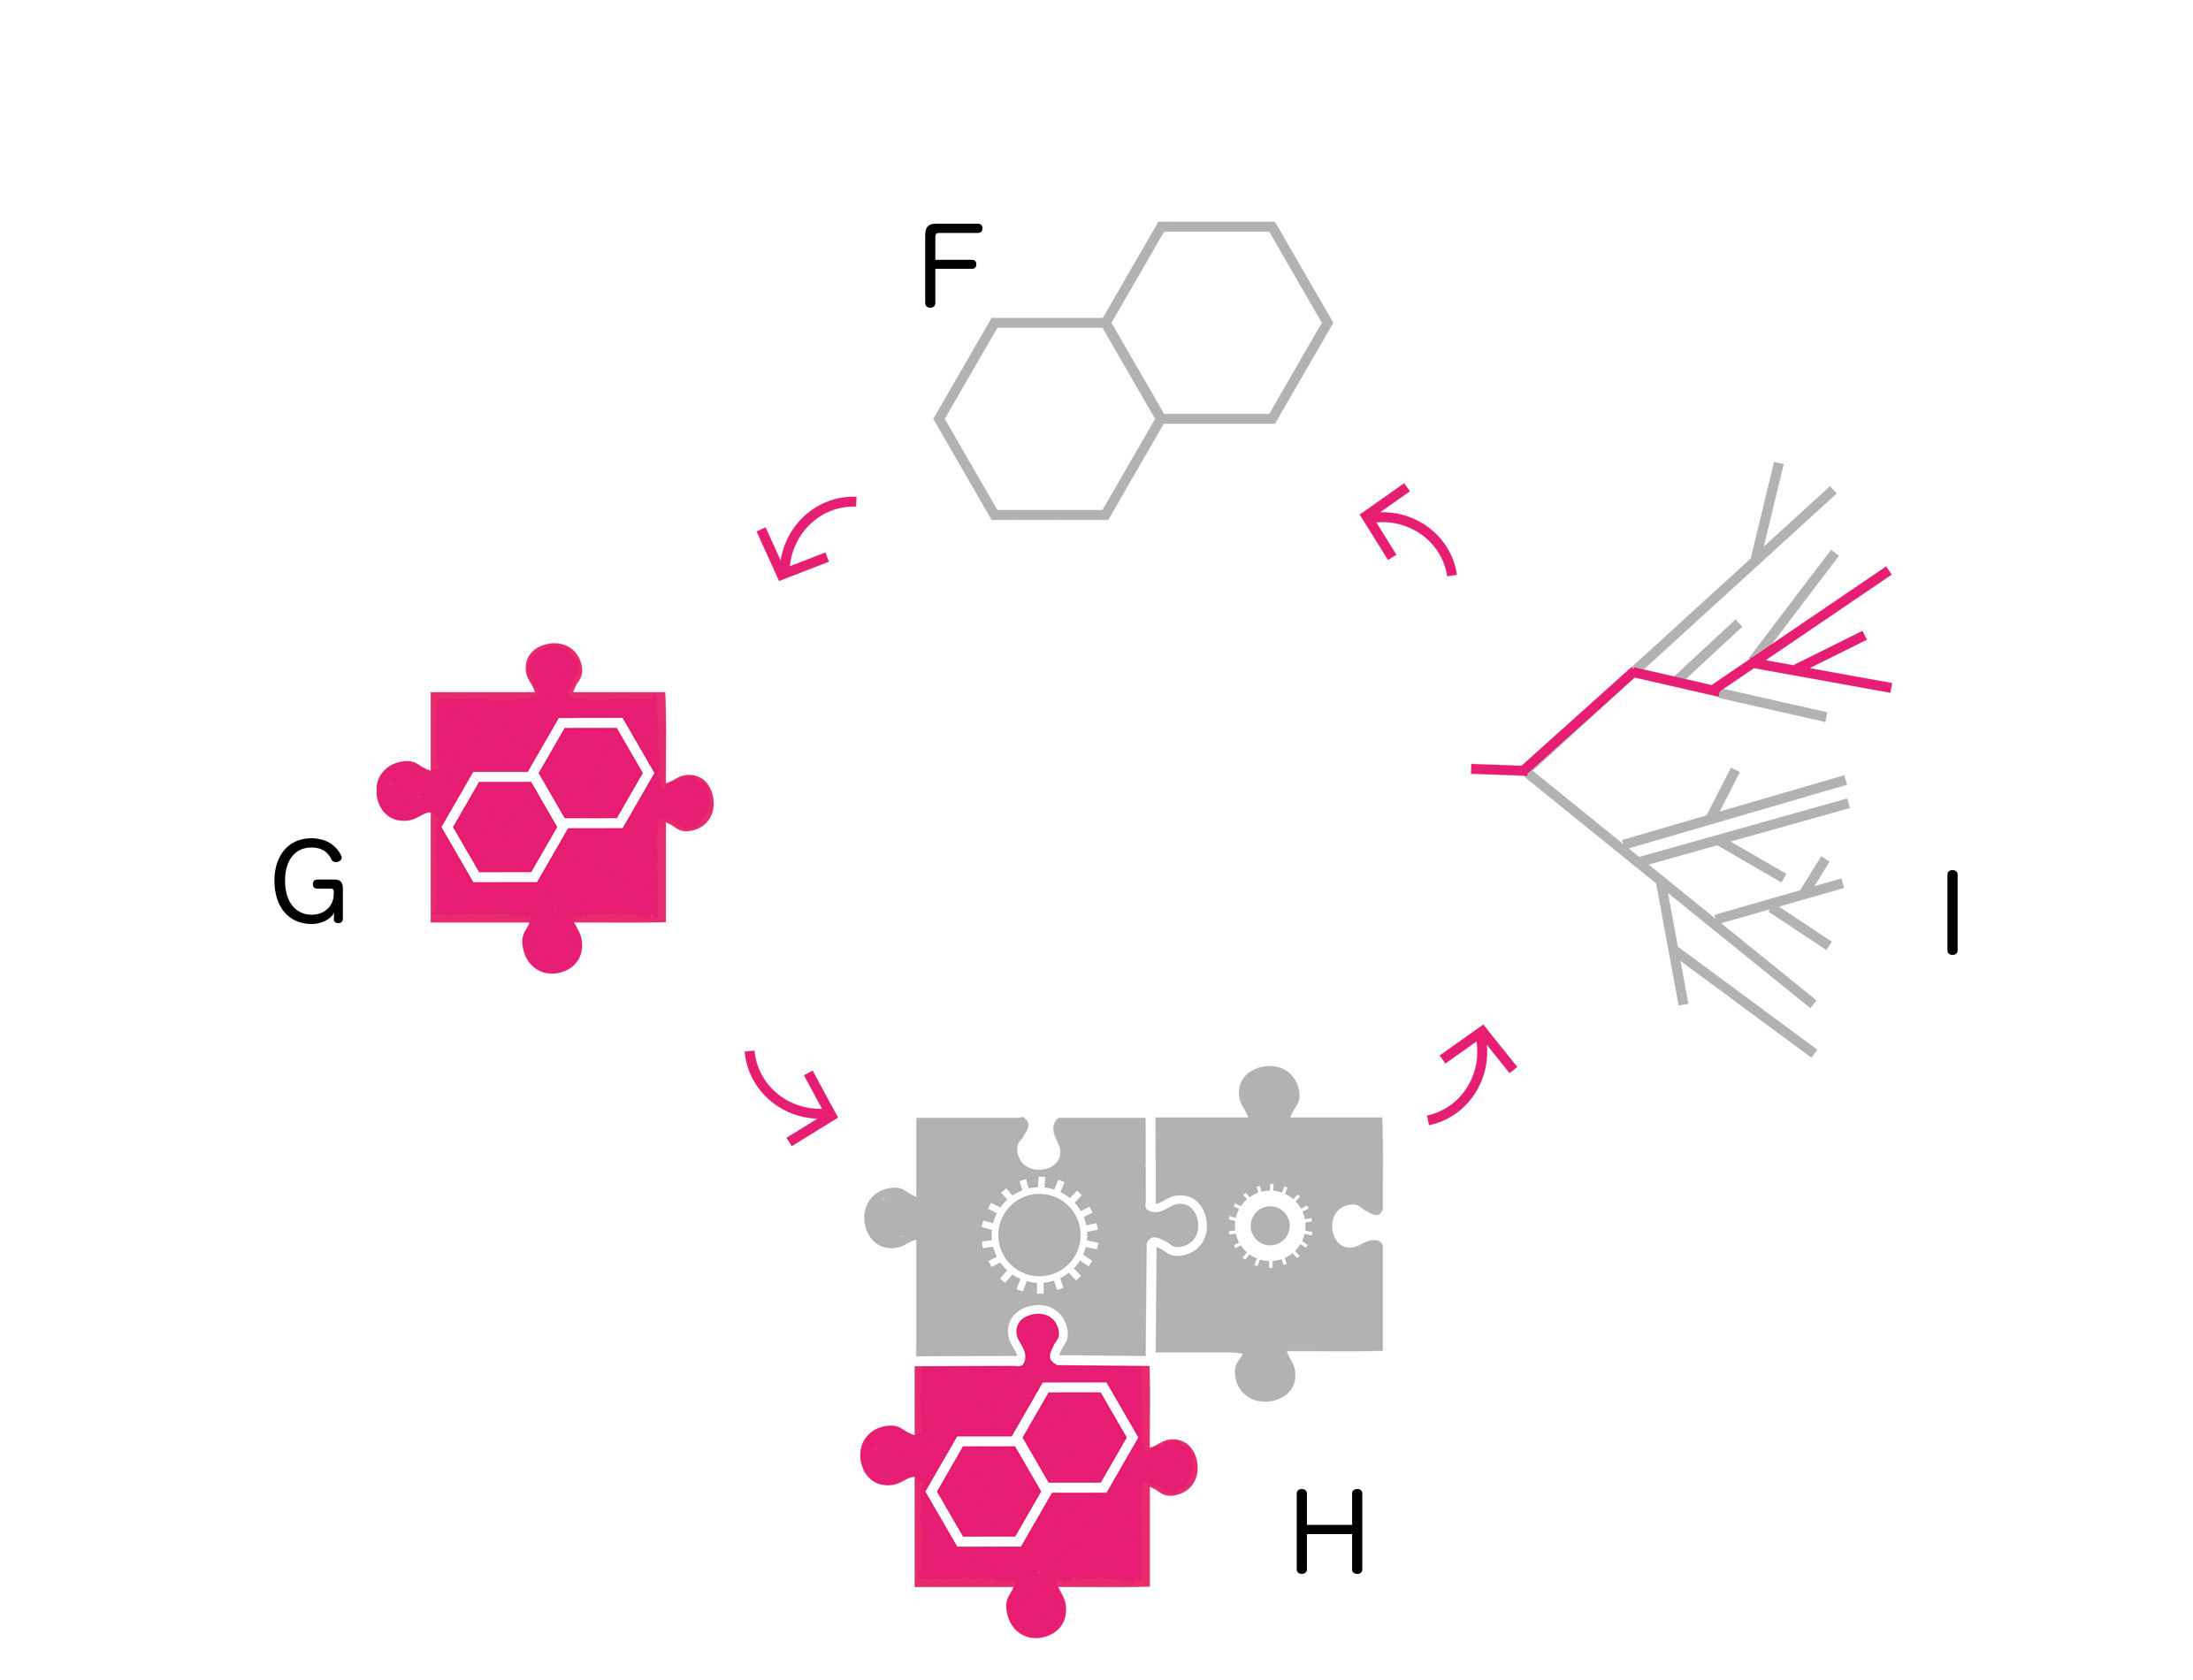
\includegraphics[scale=0.35]{nanozoo_broschuere_abwandlung_a4_part2_wletters.jpeg}\end{center}
    \caption[Infographic: Data cells are components that connect to downstream analysis pipelines.]{Data cells are components that connect to downstream analysis pipelines. A composite of data cells (F) can be plugged into downstream analyses (H) via zoo's API (G). Results from analyses such as sequence alignments or phylogenetic trees can be effectively stored in the data cell (I).}
    \label{fig:nz2}
\end{figure}


Raw sequence is annotated and analyzed with the analysis being integrated in the dataset. Consequentely, the more cyles a data set undergoes, the more curated is its content, and the more value is added to it.


\begin{figure}[H]
    \begin{center}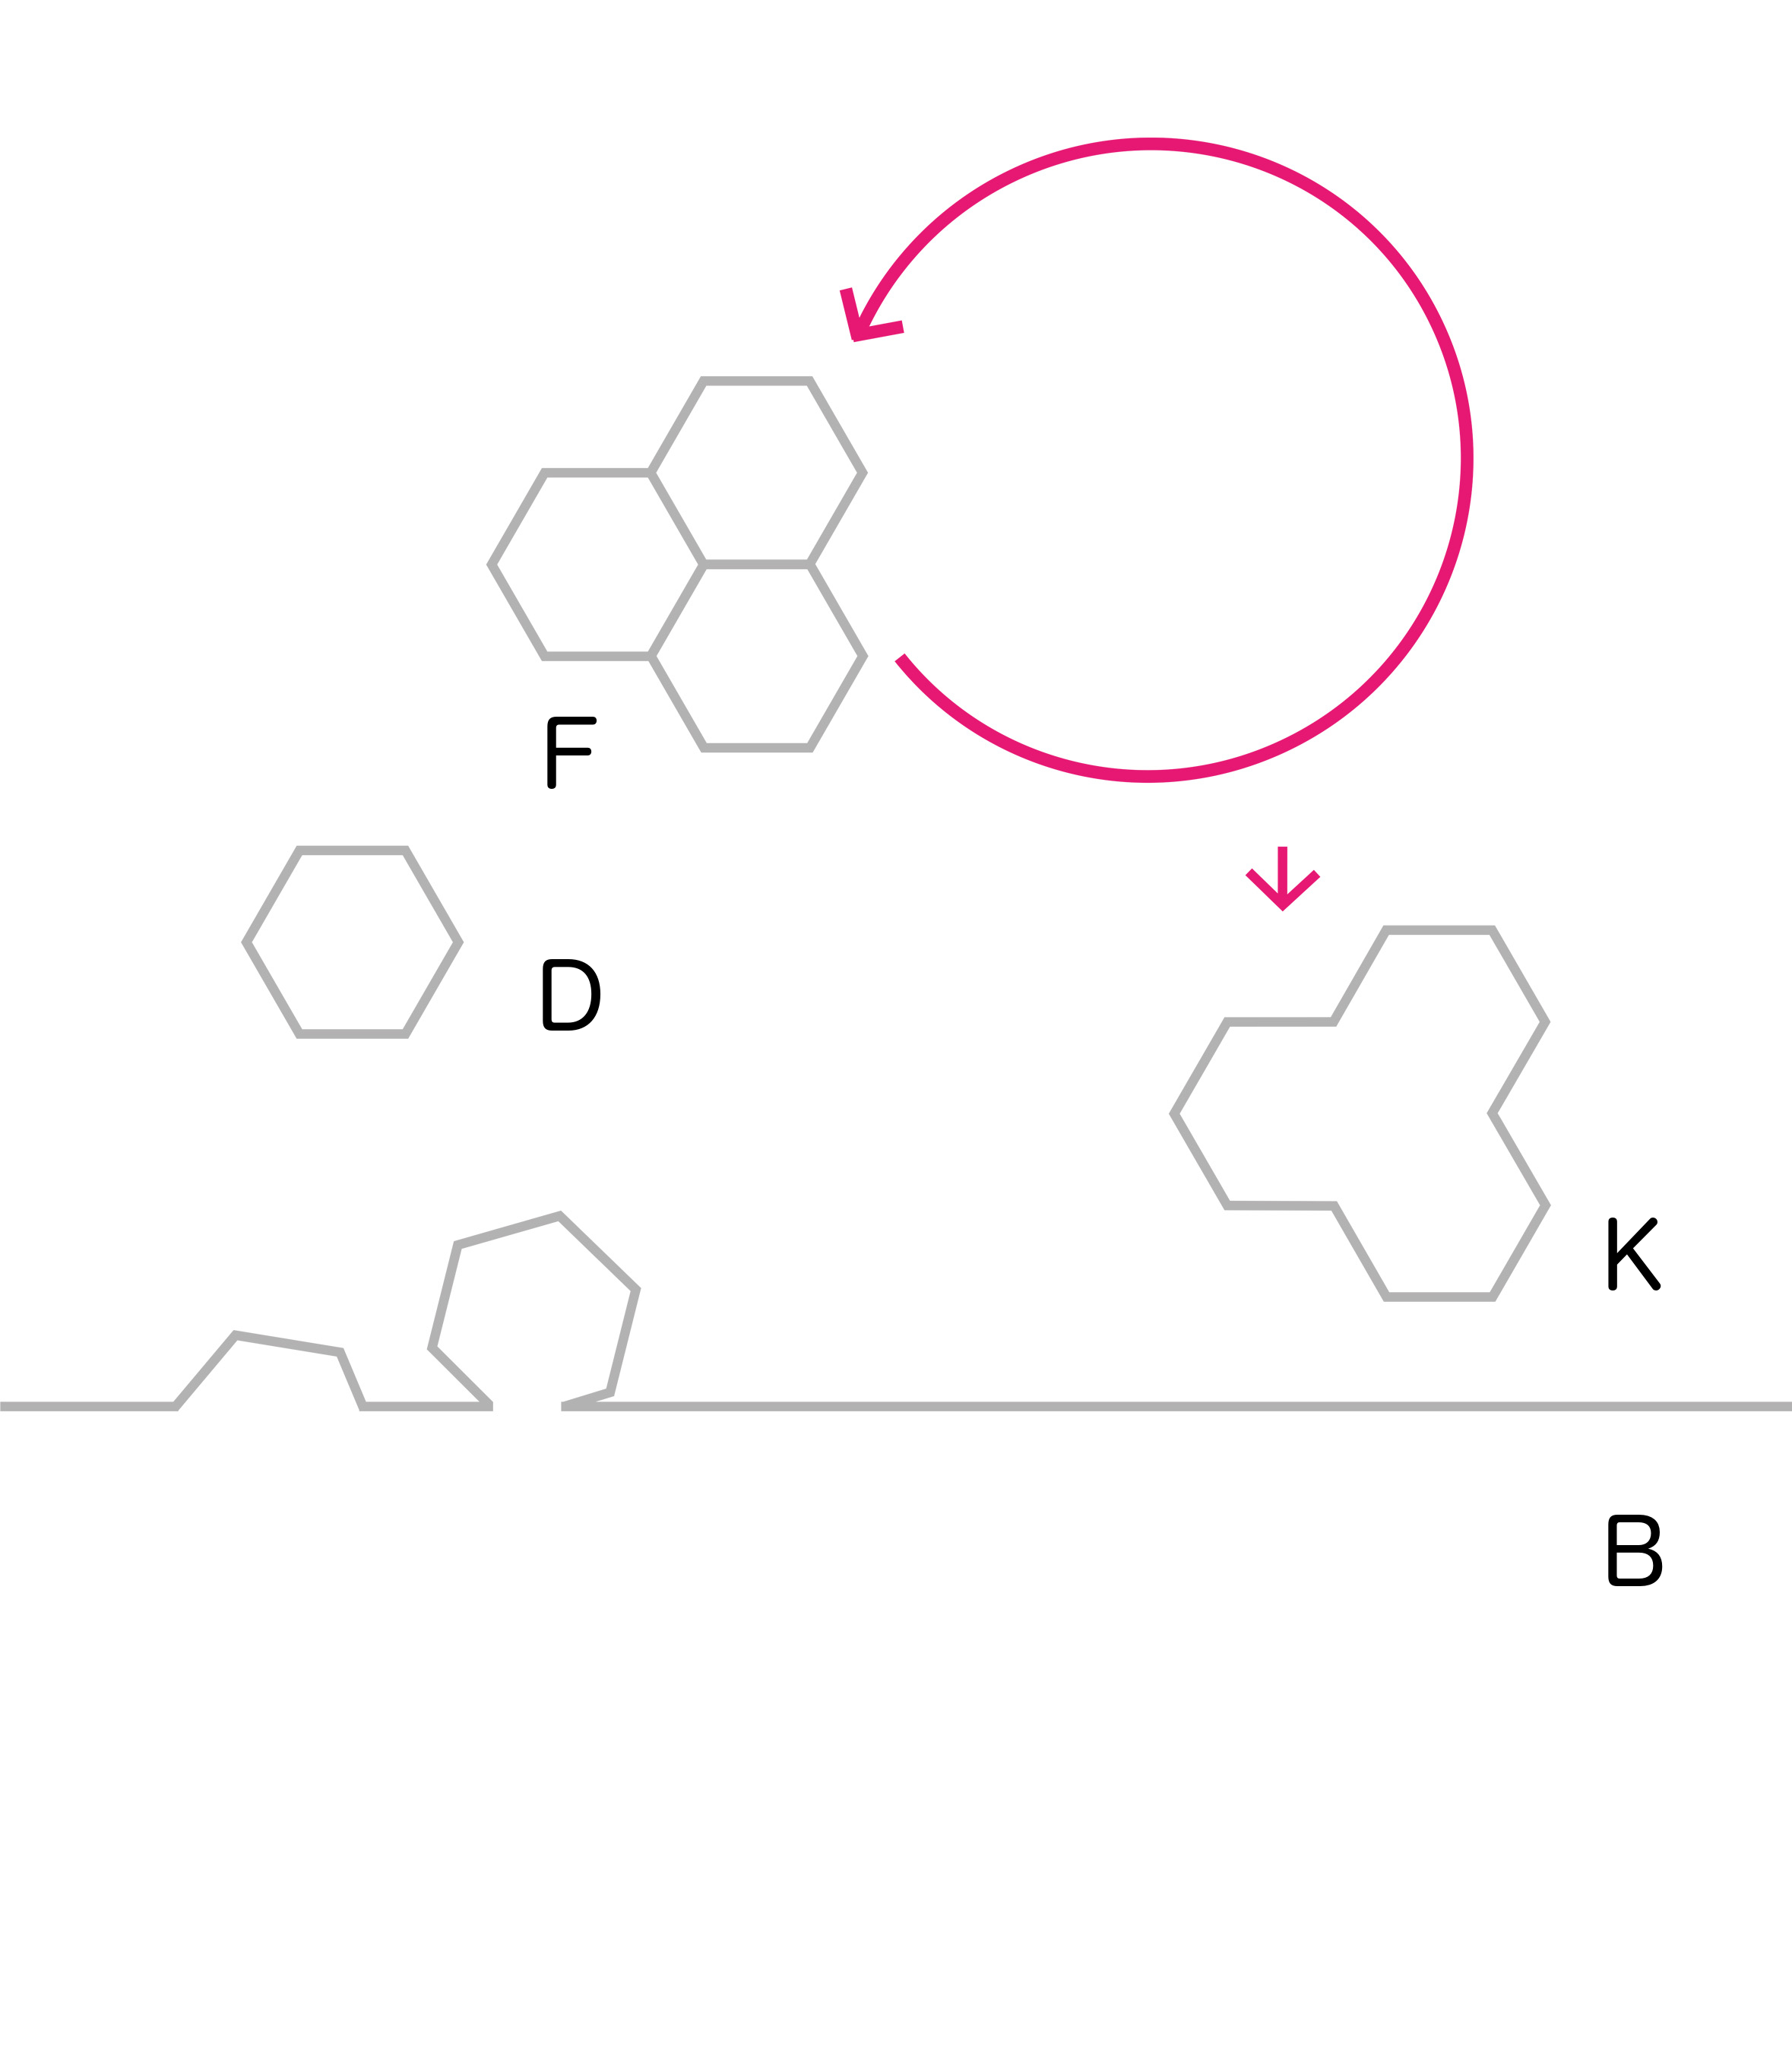
\includegraphics[scale=0.25]{nanozoo_broschuere_kreislauf_wletters.jpeg}\end{center}
    \caption[The data cycle.]{The data cycle. Data cells (D) ultimately constitute themselves in great part through public databases such as NCBI or EBI's ENA (B). They are then used as backends for analyses and store the results, which can be seen as a form of curation (F). After curation, the enhanced data is reintegrated into the public databases.}
    \label{fig:circle}
\end{figure}


From a more low-level perspective, zoo implements 4 activities on data: compose, manipulate, recycle and share.


\subsubsection{zoo: Compose}

A zoo database corresponds to a set of data cells. A data cell is a collection of documents (in NoSQL terminology). A document is a lightly structured nested hash map, typically transmitted in JSON format, a convention that zoo adopts as well. A document is composed of several schemas. These are predefined document components or templates, whose structure can be validated. For example, it can be checked whether an Influenza A virus document about to be inserted in a data cell has a correct strain nomenclature and whether a given segment is numbered from 1 to 8 or null. Because validation occures at the level of schemas, the whole database is valid by extension.

A small collection of schemas - both generic and specific to virus groups - can be found in the zoo documentation linked above. As an example, we specify here a full \gls{iav} schema composed of 5 schemas. For detailes documentation see \\ \hyperlink{https://github.com/viehwegerlib/zoo/tree/master/zoo/schema}{github.com/viehwegerlib/zoo/tree/master/zoo/schema}.


\begin{itemize}
    \item The minimum viable document in zoo is structured by a ``core'' schema with two fields (a field is a key: value pair): ``\_id'' and ``seq'' for identifier and sequence, respectively. The identifier is simply a primary key of the document. ``seq'' stands for sequence and is defined as a string with an arbitrary alphabet, typically RNA, DNA or protein. Although zoo was designed to work with microbes, especially viruses, it is agnostic to the origin of the sequence data, and as such can be used to model genomic complexities such as multiple isoforms and segmented genomes
    \item ``Metadata'' describe the way a sequence ``came to be known''. Where was it sampled from, who by, from which host, through which sample preparation and sequencing methods?
    \item The ``relative'' field includes taxonomic, phylogenic and linked information. It adresses how a given sequence compares to others. Alignments and phylogenetic trees are archived here.
    \item The ``derivative'' field summarizes or reexpresses the sequence information, e.g. via annotations, minhashes and alternative encodings like bracket-dot notation for secondary structures. Derived information is usually heavily dependent on the original sequence. For example, the annotation ``\gls{orf}'' derives from the sequence's start and a stop codon position.
    \item A (virus) specific schema, which in the case of IAV deals with some aspects of the genome structure (number and naming of segments) as well as nomenclature.
\end{itemize}

Note that all subschemas listed here are interacting: We could for example use Minhash signatures (derivative) to compare a sequence to other ones in the database, storing the result in a new field (relative).

Schemas can be composed. zoo implements a convenient notation to compose an arbitrary number of schemas in a nested document. For example, to nest metadata and annotation schemas in a core schema, we could write the following using zoo’s CLI:


\begin{lstlisting}[language=bash]
    zoo schema (core(metadata,annotation)) > schema.json
\end{lstlisting}


We can then validate records when we init/ add/ commit/ pull a data cell (see the zoo documentation for details), making sure they conform to the schema we specified earlier:


\begin{lstlisting}[language=bash]
    zoo init [...] --validate schema.json record.json
\end{lstlisting}


This makes for very flexible data entry. Instead of having a stiff format like a Genbank file we can construct hierarchical documents from prespecified components. Those are either adopted from the zoo repository or specified by the user.

On the side, this design addresses another issue: Because viruses are so diverse, it is difficult to specify a general schema that would do justice to all virus instances, past, present and future. With components, more general schemas like ``core'' and ``metadata'' can be composed with highly virus-specific ones, allowing a document to reflect nature instead of nature having to be coerced into a fixed document structure.

zoo offers many functions that facilitate work with nested hash maps, which is usually not provided out-of-the-box by many programming languages. See the docstrings of \colorbox{red-very-light}{\lstinline{zoo.utils.deep_set}} and \colorbox{red-very-light}{\lstinline{deep_get}} for examples.

zoo’s interface mostly encapsulates data. Within reason, it tries to expose data changes through common, standardized and tested operations, such as retrieving a sequence given annotation ranges. While zoo’s interface - i.e. its \gls{cli} and library (API) - handle schema composition and validation as well, its main value proposition lies in the activities of data manipulation, recycling and sharing.


\subsubsection{zoo: Manipulate}

From a practical viewpoint, working with virus data is tedious. That is not to say that people working with bacterial or human genomes are not to be pittied, but the sheer complexity and messiness of viral data is staggering. One of the problems is a lack of standardization, both in terms of taxonomy~\cite{Simmonds2017-sc, Calisher2016-mb, Simmonds2017-wj} as well as in terms of metadata. One usually has to assemble sequence data from various sources, complement annotations from another set of sources and hack together metadata based on incomplete records from a third set of sources. A tremendous amount of love and energy can flow into such curation. zoo assists with tools that make it bearable to structure data consistently in a document.

Because it runs on MongoDB, zoo supports complex queries of the form: \emph{All segments of virus X from 2007 onwards in a 500 km perimeter of Jena linked to Mosquito hosts, with sequences restricted to annotation Y and sequence similarity to some reference strain Z.} Furthermore, functions are implemented that allow the (stratified) sampling of documents based on metadata. Annotations can be quickly applied to the embedded sequence fields, and exported into a variety of formats. Furthermore, a larger part of the zoo library deals with the munging of data into e.g. binary feature matrices, which are directly compatible with standard machine learning and artificial intelligence libraries such as Scikit-learn~\cite{Pedregosa2011-yy}, Keras~\cite{Chollet2015-km} and Edwardlib~\cite{Tran2017-mc}. The overall aim is to minimize the time from input to analysis prototype.

For example, the creation of the following figure from data import to visualization took the author under 10 minutes to create. Note that the data had to be assembled from 4 different files in as many formats.


\begin{figure}[H]
    \begin{center}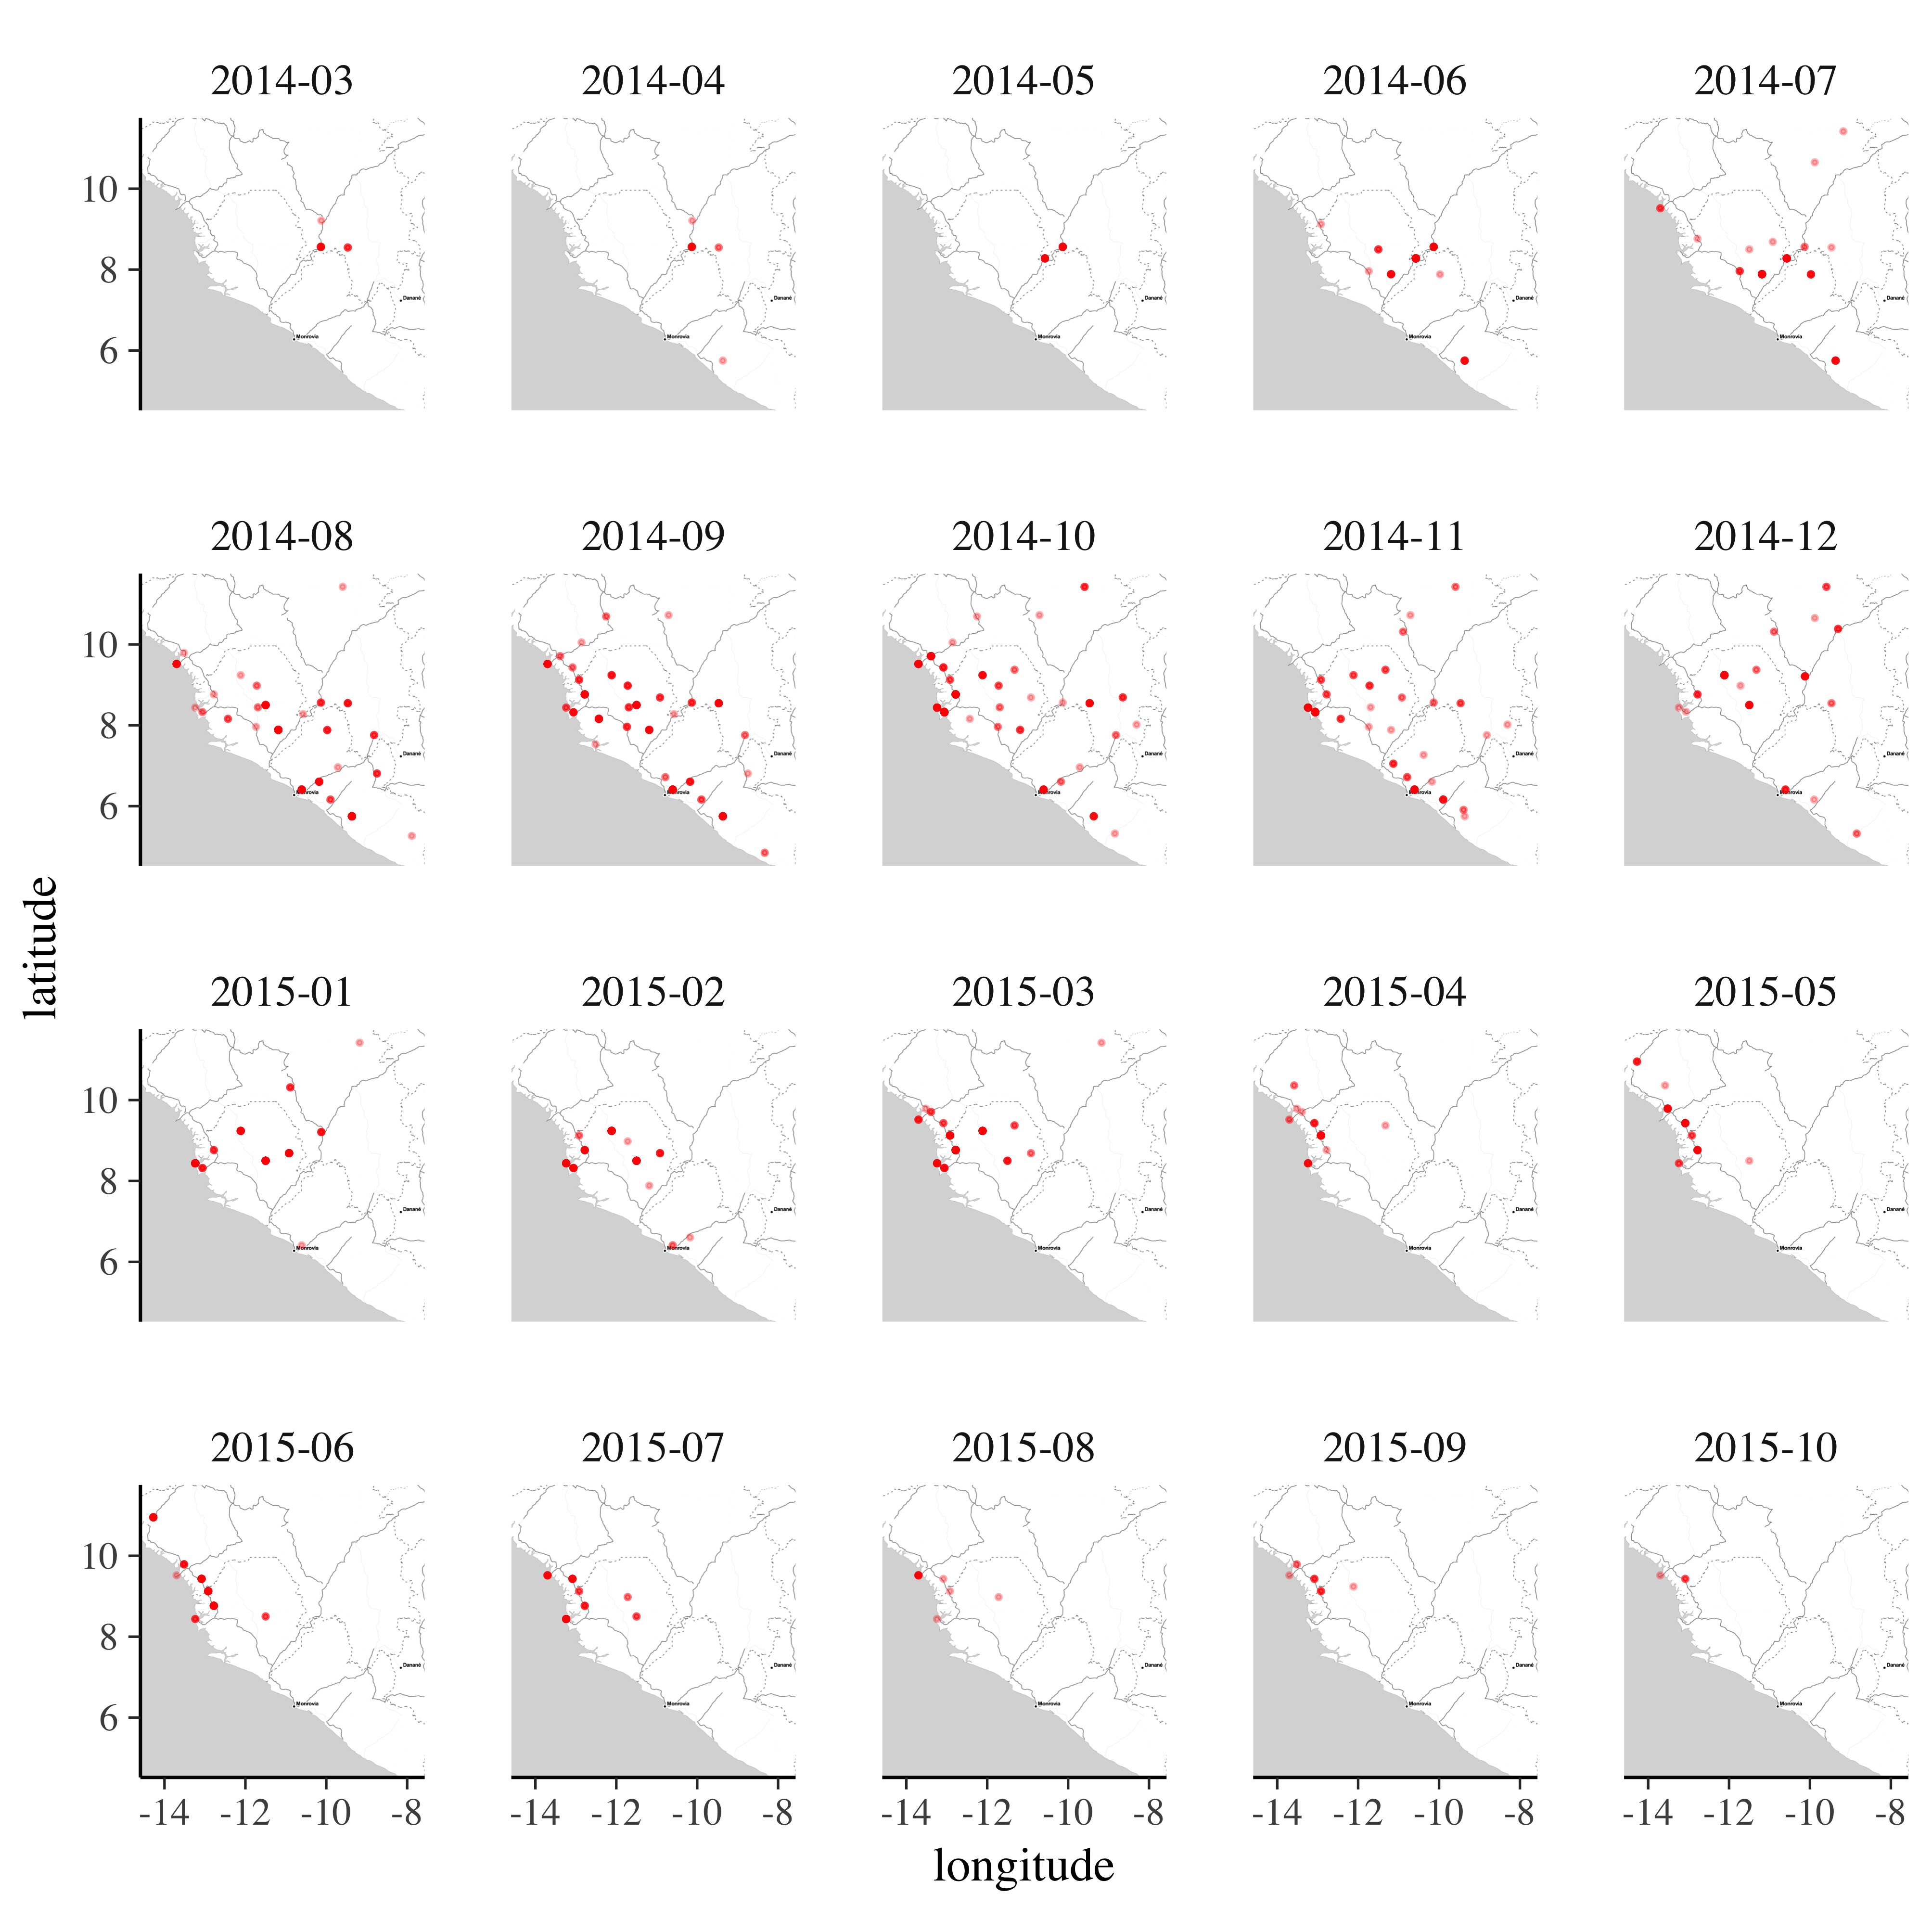
\includegraphics[scale=0.1]{makona.png}\end{center}
    \caption[Map illustrating the spatio-temporal progression of the Ebola epidemic.]{Map of the progression of the Ebola epidemic in small multiples (one for each month). Each red dot indicates a new case of Ebola. The map roughly spans West Africa, mainly Sierra Leone, Guinea and Liberia, where most Ebola cases of the outbreak 2014 - 2016 were located.}
    \label{fig:makona}
\end{figure}


\subsubsection{zoo: Recycle}

Running the same or slightly similar analysis more than once can be extremely wasteful. For example, if we computed an MSA already, it is not necessary to recompute it the moment we want to add another sequence. However, many times the first calculation is not available anymore or has a header that we slightly want to change the second time, and we end up recomputing everything. This is a wasteful practice.

zoo provides a set of functions under the title of ``digest'' (see the CLI documentation for \colorbox{red-very-light}{\lstinline{zoo digest [...]}}). They allow the decomposition of sequence alignments and tree structures into their constituents, which are then saved in the corresponding sequence’s document. For example, for an alignment an index of the loci where gaps have been inserted is stored under the ``relative'' field, together with a hash of the entire MSA. When we add new sequences to a data cell and want to extend the MSA with them, we simply reconstruct the initial MSA from the hash and gap index. We can freely modify the header format as well, because all the metadata is present in the document.

In the case of trees, zoo saves each leaf together with the path to the root in the corresponding sequence’s document. This is somewhat inefficient as we store internal nodes in many copies across multiple documents. However, we can then reconstruct the tree even though some documents might be missing.

Because zoo only works on data though its interfaces such as digest, the user is free to use whichever analysis programs she prefers. All that is required is that the output conform to standard bioinformatic formats that can be digested by and imported into zoo.


\subsubsection{zoo: Share}

zoo data cells are exported (``dumped'') to flat, human readible files in newline delimited JSON format, with one line per document. There is no prefixed header so this format is compatible with streaming applications.

These flat files are intended to be shared via \gls{p2p} networks such as Dat or IPFS, but are not limited to this. For axample, one could simple zip the dump and send it via FTP. P2P networks offer several desirable properties for information storage such as redundance, download speed and implicit version control, all of which have been adressed in the methods section.

Currently, data cells are primarily shared with the Dat protocol.


\subsubsection{Example}

To make the above explanations more concrete, we present an introductory code example that should illustrate some of zoo's command line functionalities.


\begin{minipage}{\linewidth}
\begin{lstlisting}[language=bash]

    # Create a JSON schema from zoo's templates to validate any data cell insertions.
    zoo schema (core(metadata(influenza),annotation)) \
    > schema.json
    # Or use your own.
    zoo schema --fp path/to/file (a(b,c)) > schema.json

    # Stream GenBank records to data cell, and validate schema.
    zoo load --source ncbi --fmt json \
    --ids accessions.txt --stdout - | \
    zoo init --db mockA --cell foo --validate schema.json -
    # ... Initializing data cell.
    # ... 42 entries inserted into cell "original".
    # ... Primary key assigned to field "_id".
    # ... inspect cell and commit

    zoo status --db mockA --cell foo --example

    # Make and commit changes (like you would with Git).
    zoo commit --db mockA --cell foo original
    # ... Dumping data cell.
    # ... Minhash signature computed for molecule type: DNA
    # ... | 42 Elapsed Time: 0:00:00
    # ... Done.
\end{lstlisting}
\end{minipage}


Sharing the created data cell is done over the Dat protocol. IPFS support is under development.


\begin{minipage}{\linewidth}
\begin{lstlisting}[language=bash]
    # share
    mkdir send
    cp original.json send/
    dat share send/
    # ... Syncing Dat Archive: .../send
    # ... Link:
    # dat://73401e1b931164763eccsomelonglinkcefc718ebf49f6b4fe4dbad7

    # In a faraway place, our collaborator (B) clones a copy of our
    cell and adds it to her "zoo" of other data cells.
    mkdir receive
    dat clone <link> receive/
    zoo add --db mockB --cell foo --primkey genbank.accession \ receive/original.json
    # ... Loading data cell.
    # ... Index created on field "genbank.accession".
    # ... 39 documents inserted in cell "foo".
    # ... 3 duplicates skipped.

    # Meanwhile, original.json was modified. B want his zoo to reflect
    # the changes:
    dat pull receive/
\end{lstlisting}
\end{minipage}


zoo supports commands known from the Git version control software, such as diff and pull.


\begin{minipage}{\linewidth}
\begin{lstlisting}[language=bash]
    # diff it
    zoo diff --db mockA --cell foo bar.json > diff.json
    # ... Searching for changes (delta).
    # ... Done.
    # We can pipe this, too.
    zoo diff --db mockA --cell foo bar.json | head -n2
    # Apply changes to data cell.
    zoo diff --patch --db mockA --cell foo diff.json
    # ... Loading and applying delta.
    # ... Done.

    # pull
    zoo pull --db mockB --cell foo receive/modified.json
    # ... Updating cell's md5 hashes.
    # ... / 0 Elapsed Time: 0:00:00
    # ...
    # ... 38 entries unchanged.
    # ... 4 entries replaced.

\end{lstlisting}
\end{minipage}


Two features other data structures do not offer is the reintegration of computed results with the ``digest'' command as well as support for probabilistic data structures (Minhash, SBT).


\begin{minipage}{\linewidth}
\begin{lstlisting}[language=bash]
    # Now put data cells into your favourite analysis workflow,
    # then use zoo's API to import/ export the results, like
    # multiple sequence or reference-based alignments, phylogenetic
    # trees, secondary structure ... happy exploratory
    # data analysis. Also, set global vars to reduce typing.
    ZOODB=mockB
    ZOOCELL=foo
    zoo digest --encode tree.nexus
    zoo digest --decode msa.mafft.fa

    # Not yet implemented: Send metadata about cell to a registry,
    # so others can discover it.
    zoo push ...

    # Create a sequence Bloom tree (SBT) from the minhash
    # signatures of a given cell.
    zoo sbt_index --db ref --cell virus --ksize 16 --nsketch \
    1000 virusref
    # ... Initialize SBT.
    # ... Compute minhash signatures for selected documents.
    # ... k-mer size: 16, sketch size: 1000
    # ... \ 9158 Elapsed Time: 0:01:45
    # ... Save SBT.
    # ... Done.

    # Use sourmash_lib to query other signatures about the
    # cell's SBT.
    sourmash sbt_search --ksize 16 virusref query.fa.sig
    # ... running sourmash subcommand: sbt_search
    # ... loaded query: survey.fa... (k=16, DNA)
    # ... 0.11 0ef85591-d464-4953-915f-f673907b7e8e
    # (here Zika reference genome)
\end{lstlisting}
\end{minipage}


Furthermore, zoo handles input and output in a way that is convenient and integrates well with UNIX pipelines (pipes etc.).


\begin{minipage}{\linewidth}
\begin{lstlisting}[language=bash]
    # Export, e.g. to fasta, JSON or stdout.
    zoo dump --query q.json --selection \
    _id,meta.date,meta.geo.cou,seq \
    --delim "|" --fmt fasta dump.fa

    zoo dump --query q.json --selection _id,seq \
    --fmt fasta - | head

    # Pipe into sourmash.
    zoo dump --query q.json --selection _id,seq --fmt fasta - | \
    sourmash compute -k 16 -n 100 --singleton --out q.sig -

    # Done, lets get some coffee.
    zoo drop --db mockB --cell foo --force
    zoo destroy --db mockB --force
\end{lstlisting}
\end{minipage}


\subsubsection{Scaling}

How does zoo scale? First, we need to think of what actually needs scaling, which are basically two things: The database size (including query speed) including the associated storage capacity as well as zoo’s core functionalities, such as Minhash.

A data cell can be moved to a larger compute environment if local resources are not sufficient anymore. Note however that we can load all available Influenza A virus sequences (> 700 k) from a Fasta file in less than 10 min, and query them in subsecond time on a typical laptop.

zoo's (database) engine is provided by MongoDB, the de-facto industry standard in NoSQL databases. MongoDB is known to be highly horizontally scalable to millions of documents. Cloud computing offers the required infrastructure, should the local capabilities run out. The P2P filesystem should not constitute a storage bottleneck, especially if financial incentives such as ``filecoin'' are introduced successfully.

One of the next milestones of zoo is to make the software available through a virtual machine container such as Docker or rkt. This makes the transfer to larger compute environments much easier.


\subsubsection{Integration of Minhash and SBT functions}

As described in to methods section, probabilistic data structures offer powerful ways to process large amounts of data partly with very limited resources.

In the case of zoo, the main value added comes from searching large sequence collections fast - albeit approximately - for similar sequences, and doing so in a streaming data paradigm. This can be employed as both a positive or negative filter. For example, if raw reads are queried against a data cell containing all known reference genomes (currently as of 2017 there are around 700k of them), we could filter out all known reads, and assemble only unknown ones, e.g. in the context of virus discovery. We can invert this too and use a data cell with genome variants of a single species to assign a query sequence to the closest strain, e.g. when assessing reassortment in Influenza A virus samples. With zoo it becomes trivial to set up these filters.

Also, the because all sequences are unsymmetrically hashed before we query them, this paradigm can be used with sensitive data where privacy considerations are important. For example, when a data cell is committed and a metadata registry entry prepared together with the sequence minhash, the same dataset can be queried without the person on  the other end having access to the raw sequence data. In a way, zoo provides a BLAST-like search experience of the registry, without providing access to the underlying raw data, which is handled by the user herself.

\cleardoublepage\section{Discussion}


\subsection{Unsupervised Learning}

For the unsupervised clustering we were able to separate \gls{iav} sequences by their host species. In the future we will investate this further to find out how fine-grained the resulution of these clusters can be. For example, IAV's primary reservoir is thought to be wild birds which then infect (free living) domestic bird species. In our analyses, these two host groups are lumped into one, which is a crude simplification. For these experiments, we will test the \gls{tsne}~\cite{Maaten2008-we}.

Furthermore, we did not model interactions between different k-mers explicitely. For example, if a codon is mutated during deoptimization, two dinucleotides change. We will investigate these interactions through the use of probabilistic graphical models or other related techniques.


\subsection{Supervised Learning}

Our supervised machine learning approaches yielded good predictions. However, one property of the input data was not modelleld: There are large interactions between k-mers when one deoptimized a sequence. For example, by changing one position in a codon, 2 dinucleotides are changed. We will employ probabilistic graphical models to try to infer the effects of such changes~\cite{Tran2017-mc, Bishop2013-mq}. We think that this will allow more informative deoptimization simulations, which will result in better target sequences that are then tested in the laboratory. Together with the results on feature importance, we will conduct prospective deoptimization experiments to systematically screen sequence libraries for the most attenuated virus sequence. We hope that in the distant future this work could contribute to the development of new types of vaccines, especially for RNA-viruses.


\subsection{Targeted Codon Deoptimization}

In the introduction we stated the following hypothesis:

\begin{enumerate}[label=(\alph*)]
    \item \gls{iav} is host specific, but can jump the host barrier ``easily'', especially through reassortment. We suspect that there is a host-specific IAV sequence blueprint (which we'll call a ``fluprint''). This fluprint can be discovered through machine learning. Experiments that deoptimize many loci indiscriminatively will change this fluprint. We hypothesize that what these protocols really do is change a virus'es host specificity, resulting in reduced viability. This line of argument has a long history: Early vaccines were nothing but pathogens from a from close disease variant, isolated from a different host. For example, E. Jenner used the cow pox virus to immunize against the human pox virus~\cite{Riedel2005-pt}.
    \item As a side effect, this inquiry might also elucidate how IAV is able to cross species barriers so frequently. If the constructed fluprint were correct, we should find mixed ``host signals'' in sequences from IAV that are known to have crossed this barrier, e.g. isolates from humans infected with an avian influenza strain.
\end{enumerate}


Interestingly/ Sadly, hypothesis (b) was already confirmed, which we learned after carrying out initial experiments~\cite{Eng2014-ar, Eng2016-bg}. Consequently we dropped this line of investigation. The authors use the protein sequence to classify host tropism, while we worked on the nucleotide sequence. Interestingly, random forests were used for classification, which as a machine learning technique has close ties to \gls{gbt}.

Hypothesis (a) led to mixed results. We assessed deoptimized \gls{iav} genomes retrospectively. Besides a small sample ($n = 8$ including wild type) the main problem with our inquiry was the heuristic construction of the deoptimized genomes. Certain metrics were targeted during the genome construction, such as GC content and the ``amount'' of deoptimization, all of them reasonable in the light of reports in the literature. However, no systematic deoptimization was carried out.

To exhaust all combinatorial combinations of deoptimized codons is infeasible even for short viral genomes. However, a merely heuristic approach has limited scope and is unlikely to target the codons with the highest effects on virus viability. Even if by chance this should succeed, there is little more explanation as to why the deoptimized codons should effect viability other than ``Well, because they do''.

Our approach to this problem first assumes that some property of the sequences - such as their host species - is related to virus viability. We then use a \gls{gbt} classifier to learn which nucleotide positions are most important in separating the genome sequences according to this property. This approach has some advantages:

\begin{itemize}
    \item It does not rely on heuristic assumptions about particular sites in the genome and is thus less prone to systematic biases.
    \item An arbitrary set of properties can be explored, such as host species, geographic location or point in time.
    \item The result can be directly interpreted (from a statistical viewpoint) and generates biological hypotheses, that can be followed up. For example, if certain nucleotide positions hold large feature importance, we might then investigate their role in the secondary structure of the genome, and how the latter might change if we deoptimized them.
    \item The search space of which positions to deoptimize can be prioritized, targeting sites of high feature importance in decreasing order.
\end{itemize}

As concerns our current results on the available deoptimized genomes, we cannot make tested assertions about the viability of our approach, and it remains a proof of concept. In further prospective experiments, we will generate the necessary ``wet lab'' data to do so.

Another approach we will test in the future is the use of neural networks instead of GBTs. The main limitation of our approach is that a target property, such as host species, has to be selected a priori. With deep learning we will try to learn a feature embedding of the genome sequences without this.


\subsection{Limitations of zoo}

zoo exposes many technical details to the user. In the future it will provide more abstractions to simplify the user interface. This will allow people from less technically minded backgrounds to use the software too.

Currently zoo does not address curation explicitely, i.e. it is not possible to systematically query a given dataset by curation status, such as "hand-crafted" our "automatic". Furthermore, authentication and right restrictions are not implemented. These points will be addressed once the underlying engine is robustly implemented.

Although we were able to mitigate many of the shortcoming of relational databases, mostly concerning the rigid schema they are designed around, MongoDB did present its own limitations.

The maximum document size is 16 mb, which means that for any sequence data above the size of viruses it is not possible to embed the sequence data in the document. However, by using linked information we were able to mitigate this with only a small performance cost. We did not use MongoDBs GridFS feature, which allows to store arbitrarily large blobs of binary data, because we did not want to add yet another format to the multitude of bioinformatic formats already in existence and in use in zoo. Because many formats can be indexed, lookup scales linearly, so the need to use GridFS was not apparent.

In order to allow efficient updates to the database, we used a diff-based approach, which means that only changes to documents are exchanged and applied. This approach proved brittle in cases where to much flexibility was allowed in the JSON schema, because the diff algorithm did not cover certain edge cases. In the future we will adopt a fact-oriented approach (see below) which allows efficient communication of changes without sending diffs.

There are many formats that transmit data over some wire. Most popular among them in the realm of computational biology are arguably XML and JSON. We decided to use the latter due to its wide adoption and its readibility. We also wanted to allow streaming in our communication protocols, and newline-delimited JSON allows that because there is no in-band schema or header transferred.

However, JSON is a very limited format in that it is not extendible, which means that it supports only a handful of types. Dates, sets and more arbitrary types cannot be encoded in the format. The correct usage of these fields requires context.


\subsection{tripl: A Refactoring of zoo's Database Functionality}

The refactoring of zoo's data management is called ``tripl'' and is a joint development effort with C. Small of the Fred Hutchinson Cancer Research Center, Seattle, US \\ (\hyperlink{https://github.com/metasoarous/tripl}{github.com/metasoarous/tripl}).

The tripl data format for ``all the things'', inspired by the Datomic database and the Semantic Web that has:

\begin{itemize}
    \item explicit, global meaning and context
    \item an easy document-store like write semantic
    \item capable of expressing arbitrary graph data
    \item is extensible and polymorphic
    \item primarily targets JSON for reach and interoperability
    \item theoretical underpinnings in RDF, with a simpler data-oriented buy-in model
\end{itemize}

Tripl can be created and used from any language with a natural interpretation of JSON data. However, getting the most out of the implied graph structure of the data requires some tooling - though not much: The first passable version of this tool was only 120 lines of (Python) code. Tripl's aim is to solve this problem via a minimally constrained JSON usage pattern.

Every entity must have a globally unique identity, represented as a string, typically either a namespaced keyword, a UUID, or a URI.

Every entity can be asserted via \colorbox{red-very-light}{\lstinline{db:ident}} in a dictionary/ hash map form.

If a dictionary/ map is asserted without a globally unique identity, a random UUID will be assigned.

Attributes should be namespaced keywords:

\begin{itemize}
    \item ``name'' means nothing as an identifier if used variously among different dictionaries/ maps in different places
    \item ``person:name'' and ``company:name'' as attributes unambiguously describe what their corresponding values mean, independent of the context of the corresponding entity
\end{itemize}

Values must also be serializable and hashable in JSON and any languages used to interact with the data.

Tripl is designed so that any database engine that can query a graph-like data model can be used as a backend.

\cleardoublepage\section{Summary}

Emergent infectious diseases are a growing problem due to changes in our modern environment. Yet, as the Ebola epidemic of 2014 - 2016 in Western Africa has shown, we are ill-prepared, mainly because of two shortcomings: First, we have no vaccine for many of the (especially viral) emergent diseases such as Nipah, MERS and Lassa virus. Second, our way to exchange and curate information is very inefficient, leading to large delays between data generation and action upon that data: For example, the first comprehensive analysis of the spacio-temporal dynamics of the Ebola outbreak took over a year to complete.

Engaging the first problem, a technique called ``codon deoptimization'' is promising to generate live vaccines quickly and in theory for arbitrary viruses. We applied machine learning to help make the design of deoptimized vaccine candidates more informed and thus effective.

To encounter the second problem we designed and implemented a new data structure and exchange protocol. It serves as a proof of concept and illustrates how such structures can dramatically shorten the time from data to action, which is of vital importance in the context of public health surveillance.

\cleardoublepage\section{Epilogue}

\begin{quotation}
    \emph{What about the future? It doesn't take a rocket scientist to work out we are going to get more infections in the future. This is really obvious. Animals carry an enormous number of pathogens that can jump into humans. The way we live today - we have cut down forests, we have changed farming, big cities, international travel - they just fuel the engine of viral emergence and evolution. How do we prevent this? [...] Some people say: Well, let's try and predict what is going to emerge. Let me tell you, just - forget that. Ok? [...] You can't predict what is going to emerge. [...] And I also don't think that just going out into nature and surveilling things is going to be the answer, because there are millions of things out there. Response is better than prediction. [...] And we have the tools: What's called metagenomics [...] can save the planet. -- \hyperlink{https://www.youtube.com/watch?v=iK8ekVy_rmQ}{E. Holmes}}
\end{quotation}



% https://www.sharelatex.com/learn/Bibtex_√bibliography_styles
\cleardoublepage\bibliography{lib.bib}{}


\cleardoublepage\section{Appendix}

The accompanying code and documentation can be accessed from the following repositories:

\begin{itemize}
\item https://github.com/viehwegerlib/master-thesis
\item https://github.com/viehwegerlib/zoo
\end{itemize}

A copy of the code is provided on a USB stick.

``Code'' refers to the following items:

\begin{itemize}
    \item the LATEX code that generated this thesis including the images
    \item codon-based \gls{msa} script
    \item deoptimized sequence data (provided by D. Kunec)
    \item code to transform sequences for machine learning algorithms
    \item machine learning code including parameter tuning and testing
    \item code for genome clustering experiments
    \item the zoo package
\end{itemize}

\cleardoublepage% Disclaimer ====================================================================

\vspace*{\fill}
\begin{center}
Ich versichere, dass ich die vorliegende Arbeit selbständig und nur unter  Verwendung der angegebenen Quellen und Hilfsmittel angefertigt habe, insbesondere sind wörtliche oder sinngemäße Zitate als solche gekennzeichnet. Mir ist bekannt, dass Zuwiderhandlung auch nachträglich zur Aberkennung des Abschlusses führen kann.

\vspace{3cm}

Leipzig, \selectlanguage{german}\today \hfill Unterschrift
\end{center}
\vspace*{\fill}
\vspace*{\fill}
\vspace*{\fill}



\end{document}
